% Options for packages loaded elsewhere
\PassOptionsToPackage{unicode}{hyperref}
\PassOptionsToPackage{hyphens}{url}
%
\documentclass[
]{book}
\usepackage{amsmath,amssymb}
\usepackage{lmodern}
\usepackage{ifxetex,ifluatex}
\ifnum 0\ifxetex 1\fi\ifluatex 1\fi=0 % if pdftex
  \usepackage[T1]{fontenc}
  \usepackage[utf8]{inputenc}
  \usepackage{textcomp} % provide euro and other symbols
\else % if luatex or xetex
  \usepackage{unicode-math}
  \defaultfontfeatures{Scale=MatchLowercase}
  \defaultfontfeatures[\rmfamily]{Ligatures=TeX,Scale=1}
\fi
% Use upquote if available, for straight quotes in verbatim environments
\IfFileExists{upquote.sty}{\usepackage{upquote}}{}
\IfFileExists{microtype.sty}{% use microtype if available
  \usepackage[]{microtype}
  \UseMicrotypeSet[protrusion]{basicmath} % disable protrusion for tt fonts
}{}
\makeatletter
\@ifundefined{KOMAClassName}{% if non-KOMA class
  \IfFileExists{parskip.sty}{%
    \usepackage{parskip}
  }{% else
    \setlength{\parindent}{0pt}
    \setlength{\parskip}{6pt plus 2pt minus 1pt}}
}{% if KOMA class
  \KOMAoptions{parskip=half}}
\makeatother
\usepackage{xcolor}
\IfFileExists{xurl.sty}{\usepackage{xurl}}{} % add URL line breaks if available
\IfFileExists{bookmark.sty}{\usepackage{bookmark}}{\usepackage{hyperref}}
\hypersetup{
  pdftitle={Introduction to Data Science in R},
  pdfauthor={Joseph M. Westenberg},
  hidelinks,
  pdfcreator={LaTeX via pandoc}}
\urlstyle{same} % disable monospaced font for URLs
\usepackage{color}
\usepackage{fancyvrb}
\newcommand{\VerbBar}{|}
\newcommand{\VERB}{\Verb[commandchars=\\\{\}]}
\DefineVerbatimEnvironment{Highlighting}{Verbatim}{commandchars=\\\{\}}
% Add ',fontsize=\small' for more characters per line
\usepackage{framed}
\definecolor{shadecolor}{RGB}{248,248,248}
\newenvironment{Shaded}{\begin{snugshade}}{\end{snugshade}}
\newcommand{\AlertTok}[1]{\textcolor[rgb]{0.94,0.16,0.16}{#1}}
\newcommand{\AnnotationTok}[1]{\textcolor[rgb]{0.56,0.35,0.01}{\textbf{\textit{#1}}}}
\newcommand{\AttributeTok}[1]{\textcolor[rgb]{0.77,0.63,0.00}{#1}}
\newcommand{\BaseNTok}[1]{\textcolor[rgb]{0.00,0.00,0.81}{#1}}
\newcommand{\BuiltInTok}[1]{#1}
\newcommand{\CharTok}[1]{\textcolor[rgb]{0.31,0.60,0.02}{#1}}
\newcommand{\CommentTok}[1]{\textcolor[rgb]{0.56,0.35,0.01}{\textit{#1}}}
\newcommand{\CommentVarTok}[1]{\textcolor[rgb]{0.56,0.35,0.01}{\textbf{\textit{#1}}}}
\newcommand{\ConstantTok}[1]{\textcolor[rgb]{0.00,0.00,0.00}{#1}}
\newcommand{\ControlFlowTok}[1]{\textcolor[rgb]{0.13,0.29,0.53}{\textbf{#1}}}
\newcommand{\DataTypeTok}[1]{\textcolor[rgb]{0.13,0.29,0.53}{#1}}
\newcommand{\DecValTok}[1]{\textcolor[rgb]{0.00,0.00,0.81}{#1}}
\newcommand{\DocumentationTok}[1]{\textcolor[rgb]{0.56,0.35,0.01}{\textbf{\textit{#1}}}}
\newcommand{\ErrorTok}[1]{\textcolor[rgb]{0.64,0.00,0.00}{\textbf{#1}}}
\newcommand{\ExtensionTok}[1]{#1}
\newcommand{\FloatTok}[1]{\textcolor[rgb]{0.00,0.00,0.81}{#1}}
\newcommand{\FunctionTok}[1]{\textcolor[rgb]{0.00,0.00,0.00}{#1}}
\newcommand{\ImportTok}[1]{#1}
\newcommand{\InformationTok}[1]{\textcolor[rgb]{0.56,0.35,0.01}{\textbf{\textit{#1}}}}
\newcommand{\KeywordTok}[1]{\textcolor[rgb]{0.13,0.29,0.53}{\textbf{#1}}}
\newcommand{\NormalTok}[1]{#1}
\newcommand{\OperatorTok}[1]{\textcolor[rgb]{0.81,0.36,0.00}{\textbf{#1}}}
\newcommand{\OtherTok}[1]{\textcolor[rgb]{0.56,0.35,0.01}{#1}}
\newcommand{\PreprocessorTok}[1]{\textcolor[rgb]{0.56,0.35,0.01}{\textit{#1}}}
\newcommand{\RegionMarkerTok}[1]{#1}
\newcommand{\SpecialCharTok}[1]{\textcolor[rgb]{0.00,0.00,0.00}{#1}}
\newcommand{\SpecialStringTok}[1]{\textcolor[rgb]{0.31,0.60,0.02}{#1}}
\newcommand{\StringTok}[1]{\textcolor[rgb]{0.31,0.60,0.02}{#1}}
\newcommand{\VariableTok}[1]{\textcolor[rgb]{0.00,0.00,0.00}{#1}}
\newcommand{\VerbatimStringTok}[1]{\textcolor[rgb]{0.31,0.60,0.02}{#1}}
\newcommand{\WarningTok}[1]{\textcolor[rgb]{0.56,0.35,0.01}{\textbf{\textit{#1}}}}
\usepackage{longtable,booktabs,array}
\usepackage{calc} % for calculating minipage widths
% Correct order of tables after \paragraph or \subparagraph
\usepackage{etoolbox}
\makeatletter
\patchcmd\longtable{\par}{\if@noskipsec\mbox{}\fi\par}{}{}
\makeatother
% Allow footnotes in longtable head/foot
\IfFileExists{footnotehyper.sty}{\usepackage{footnotehyper}}{\usepackage{footnote}}
\makesavenoteenv{longtable}
\usepackage{graphicx}
\makeatletter
\def\maxwidth{\ifdim\Gin@nat@width>\linewidth\linewidth\else\Gin@nat@width\fi}
\def\maxheight{\ifdim\Gin@nat@height>\textheight\textheight\else\Gin@nat@height\fi}
\makeatother
% Scale images if necessary, so that they will not overflow the page
% margins by default, and it is still possible to overwrite the defaults
% using explicit options in \includegraphics[width, height, ...]{}
\setkeys{Gin}{width=\maxwidth,height=\maxheight,keepaspectratio}
% Set default figure placement to htbp
\makeatletter
\def\fps@figure{htbp}
\makeatother
\setlength{\emergencystretch}{3em} % prevent overfull lines
\providecommand{\tightlist}{%
  \setlength{\itemsep}{0pt}\setlength{\parskip}{0pt}}
\setcounter{secnumdepth}{5}
\usepackage{booktabs}
\usepackage{amsthm}
\makeatletter
\def\thm@space@setup{%
  \thm@preskip=8pt plus 2pt minus 4pt
  \thm@postskip=\thm@preskip
}
\makeatother
\usepackage{booktabs}
\usepackage{longtable}
\usepackage{array}
\usepackage{multirow}
\usepackage{wrapfig}
\usepackage{float}
\usepackage{colortbl}
\usepackage{pdflscape}
\usepackage{tabu}
\usepackage{threeparttable}
\usepackage{threeparttablex}
\usepackage[normalem]{ulem}
\usepackage{makecell}
\usepackage{xcolor}
\ifluatex
  \usepackage{selnolig}  % disable illegal ligatures
\fi
\usepackage[]{natbib}
\bibliographystyle{apalike}

\title{Introduction to Data Science in R}
\author{Joseph M. Westenberg}
\date{2021-07-15}

\begin{document}
\maketitle

{
\setcounter{tocdepth}{1}
\tableofcontents
}
\hypertarget{preface}{%
\chapter{Preface}\label{preface}}

These notes are a first draft and quite prelimenary. If you find errors, please let me know by emailing \href{mailto:jwesten@iu.edu}{\nolinkurl{jwesten@iu.edu}}

An example of my code for this course is avaialabe on my github repository at \url{https://github.com/r-introtodatascience/sample_repo}.

The goal of these short courses are to give graduate students a very prelimenary introduction into coding in R. While having an `instructor' teach you these things may be helpful, in my belief, coding, like math, you have to learn by doing. So I highly encourage following these notes, but then play around with the code. Change things and see how it changes the output. I think this is the best way to learn.

Over the next 5 `sessions' we will be looking into county level unemployment data. The goal will be to provide examples and descriptions of the commands and techniques I have discovered to be most useful while working with data. Specifically the goal is by the end of the sessions it is my hope that you will know how to:

\begin{itemize}
\tightlist
\item
  download data straight into R
\item
  read in data (Rda, csv, xlsx, dta)
\item
  merge datasets
\item
  subset datasets
\item
  create summary statistics and plots
\item
  run basic regressions
\end{itemize}

all while paying particular attention to file pathing and to teach you how to export graphics and tables from R into a form that can be directly read into LaTex (so that it can be easily read into paper/presentation documents).

Below is an example of an interactive plot you can make with a package called plotly. Try interacting with it! In the plot you can select/deselect states you want to view. There is also a link to a short post I made about using GIS with R. I show these to illustrate a bit of what is possible to do in R after we familiarize ourselves with the basic functions.

\includegraphics{bookdown-demo_files/figure-latex/unnamed-chunk-2-1.pdf}

\hypertarget{intro}{%
\chapter{Introduction}\label{intro}}

The goal of this section is to provide a very quick introduction or refresher to R. If this is your first time coding, this brief introduction will most likely be quite insufficient. I encourage you to seek other resources to learn the basics before proceeding.

In particular we will cover:

\begin{itemize}
\tightlist
\item
  Writing Loops
\item
  String Manipulation
\item
  Project Organization
\item
  Downloading/Reading Data
\item
  Downloading Loop
\end{itemize}

In this lesson we will be downloading and cleaning data from the BLS on county level employment statistics from 1990-2019.

\hypertarget{very-basics}{%
\section{Very Basics}\label{very-basics}}

I assume you have R installed and running. There are plenty of guides online on how to do this.

Let's first define some arrays within R.

These can be numeric based, in this case integer.

\begin{Shaded}
\begin{Highlighting}[numbers=left,,]
\NormalTok{numvec1}\OtherTok{\textless{}{-}}\FunctionTok{c}\NormalTok{(}\DecValTok{5}\NormalTok{,}\DecValTok{6}\NormalTok{,}\DecValTok{7}\NormalTok{)  }\CommentTok{\# 1}
\NormalTok{numvec2}\OtherTok{\textless{}{-}}\FunctionTok{c}\NormalTok{(}\DecValTok{7}\NormalTok{,}\DecValTok{8}\NormalTok{,}\DecValTok{9}\NormalTok{)  }\CommentTok{\# 2}
\end{Highlighting}
\end{Shaded}

Let's dig into what is going on a bit more. We are telling R to define a vector, this is the c( ) part, with elements 1,2,3 and give that vector a name A. The backwards arrow tells R what is the name and what is the element we are defining.

We can make character based vectors as well.

\begin{Shaded}
\begin{Highlighting}[numbers=left,,]
\NormalTok{charvec1}\OtherTok{\textless{}{-}}\FunctionTok{c}\NormalTok{(}\StringTok{"a"}\NormalTok{, }\StringTok{"b"}\NormalTok{, }\StringTok{"c"}\NormalTok{)  }\CommentTok{\# 1}
\NormalTok{charvec2}\OtherTok{\textless{}{-}}\FunctionTok{c}\NormalTok{(}\StringTok{"d"}\NormalTok{, }\StringTok{"e"}\NormalTok{, }\StringTok{"f"}\NormalTok{)  }\CommentTok{\# 2}
\end{Highlighting}
\end{Shaded}

We can then combine these vectors into a dataframe (this is relevant for when we start thinking about reading in/manipulating actual data). Since all of our vectors are length three, we can easily create a dataframe (think a matrix) where our column names will be the name of the vectors, and the rows will be the elements of the vectors.

\begin{Shaded}
\begin{Highlighting}[numbers=left,,]
\NormalTok{first\_dataframe}\OtherTok{\textless{}{-}}\FunctionTok{data.frame}\NormalTok{(numvec1,numvec2,charvec1,charvec2)  }\CommentTok{\# 1}
\FunctionTok{print}\NormalTok{(first\_dataframe)                                          }\CommentTok{\# 2}
\end{Highlighting}
\end{Shaded}

\begin{verbatim}
##   numvec1 numvec2 charvec1 charvec2
## 1       5       7        a        d
## 2       6       8        b        e
## 3       7       9        c        f
\end{verbatim}

Now first\_dataframe is going to be of similar format as we will typically have when we read in data from excel files into R. We can access certain rows and columns within the dataframe by putting square brackets after the name of the dataframe. For example if we wanted to print the element in the first row and first column, we could define the variable x as this and then print x. (Keep in mind the ordering is rows, columns)

\begin{Shaded}
\begin{Highlighting}[numbers=left,,]
\NormalTok{x}\OtherTok{\textless{}{-}}\NormalTok{first\_dataframe[}\DecValTok{1}\NormalTok{,}\DecValTok{1}\NormalTok{]  }\CommentTok{\# 1}
\FunctionTok{print}\NormalTok{(x)                 }\CommentTok{\# 2}
\end{Highlighting}
\end{Shaded}

\begin{verbatim}
## [1] 5
\end{verbatim}

What if we wanted to print \textbf{all} elements in the first row, we just leave the column (after the comma) blank:

\begin{Shaded}
\begin{Highlighting}[numbers=left,,]
\NormalTok{x}\OtherTok{\textless{}{-}}\NormalTok{first\_dataframe[}\DecValTok{1}\NormalTok{,]  }\CommentTok{\# 1}
\FunctionTok{print}\NormalTok{(x)                }\CommentTok{\# 2}
\end{Highlighting}
\end{Shaded}

\begin{verbatim}
##   numvec1 numvec2 charvec1 charvec2
## 1       5       7        a        d
\end{verbatim}

How about 1st \& 3rd row?

\begin{Shaded}
\begin{Highlighting}[numbers=left,,]
\NormalTok{x}\OtherTok{\textless{}{-}}\NormalTok{first\_dataframe[}\FunctionTok{c}\NormalTok{(}\DecValTok{1}\NormalTok{,}\DecValTok{3}\NormalTok{),]  }\CommentTok{\# 1}
\FunctionTok{print}\NormalTok{(x)                     }\CommentTok{\# 2}
\end{Highlighting}
\end{Shaded}

\begin{verbatim}
##   numvec1 numvec2 charvec1 charvec2
## 1       5       7        a        d
## 3       7       9        c        f
\end{verbatim}

Another way to do this is to define another variable, say y as a vector with elements 1 and 3. Notice how the below output is the same as the above.

\begin{Shaded}
\begin{Highlighting}[numbers=left,,]
\NormalTok{y}\OtherTok{\textless{}{-}}\FunctionTok{c}\NormalTok{(}\DecValTok{1}\NormalTok{,}\DecValTok{3}\NormalTok{)               }\CommentTok{\# 1}
\NormalTok{x}\OtherTok{\textless{}{-}}\NormalTok{first\_dataframe[y,]  }\CommentTok{\# 2}
\FunctionTok{print}\NormalTok{(x)                }\CommentTok{\# 3}
\end{Highlighting}
\end{Shaded}

\begin{verbatim}
##   numvec1 numvec2 charvec1 charvec2
## 1       5       7        a        d
## 3       7       9        c        f
\end{verbatim}

We can do the same thing for the columns (we need to remember the order for the square brackets are rows, columns). Note: if we put a negative sign in front of these commands in the brackets, instead ``keeping'' certain rows or columns, it means remove! That is if in the below command we have -3, it would be saying REMOVE column 3!

\begin{Shaded}
\begin{Highlighting}[numbers=left,,]
\NormalTok{x}\OtherTok{\textless{}{-}}\NormalTok{first\_dataframe[,}\DecValTok{3}\NormalTok{]   }\CommentTok{\# 1}
\NormalTok{y}\OtherTok{\textless{}{-}}\NormalTok{first\_dataframe[,}\SpecialCharTok{{-}}\DecValTok{3}\NormalTok{]  }\CommentTok{\# 2}
\FunctionTok{print}\NormalTok{(x)                 }\CommentTok{\# 3}
\end{Highlighting}
\end{Shaded}

\begin{verbatim}
## [1] "a" "b" "c"
\end{verbatim}

\begin{Shaded}
\begin{Highlighting}[numbers=left,,]
\FunctionTok{print}\NormalTok{(y)  }\CommentTok{\# 1}
\end{Highlighting}
\end{Shaded}

\begin{verbatim}
##   numvec1 numvec2 charvec2
## 1       5       7        d
## 2       6       8        e
## 3       7       9        f
\end{verbatim}

Our third column is named C, we can also pull this column by referencing it's name after a dollar sign, such as:

\begin{Shaded}
\begin{Highlighting}[numbers=left,,]
\NormalTok{x}\OtherTok{\textless{}{-}}\NormalTok{first\_dataframe}\SpecialCharTok{$}\NormalTok{charvec1  }\CommentTok{\# 1}
\FunctionTok{print}\NormalTok{(x)                     }\CommentTok{\# 2}
\end{Highlighting}
\end{Shaded}

\begin{verbatim}
## [1] "a" "b" "c"
\end{verbatim}

This may not sound useful now, but think if we have many columns of variables, say wage, hoursworked, fulltime, and hundreds of more. We don't want to have to find what column number hoursworked is, we can just reference this column name.

\hypertarget{and-and-or-operators}{%
\subsubsection{``And'' and ``Or'' Operators}\label{and-and-or-operators}}

A couple common operators that we may want to use are ``and'' and ``or'' statements. Within R:

\begin{itemize}
\tightlist
\item
  ``\&'' : Our ``and'' operator
\item
  ``\textbar{}'' : Our ``or'' operator
\end{itemize}

For example:

\begin{Shaded}
\begin{Highlighting}[]
\NormalTok{first\_dataframe[first\_dataframe}\SpecialCharTok{$}\NormalTok{numvec1}\SpecialCharTok{\textgreater{}=}\DecValTok{6} \SpecialCharTok{\&}\NormalTok{ first\_dataframe}\SpecialCharTok{$}\NormalTok{numvec2}\SpecialCharTok{\textless{}}\DecValTok{9}\NormalTok{,]  }\CommentTok{\# 1}
\end{Highlighting}
\end{Shaded}

\begin{verbatim}
##   numvec1 numvec2 charvec1 charvec2
## 2       6       8        b        e
\end{verbatim}

\begin{Shaded}
\begin{Highlighting}[]
\NormalTok{first\_dataframe[first\_dataframe}\SpecialCharTok{$}\NormalTok{numvec1}\SpecialCharTok{\textgreater{}=}\DecValTok{6} \SpecialCharTok{|}\NormalTok{ first\_dataframe}\SpecialCharTok{$}\NormalTok{numvec2}\SpecialCharTok{\textless{}}\DecValTok{9}\NormalTok{,]  }\CommentTok{\# 1}
\end{Highlighting}
\end{Shaded}

\begin{verbatim}
##   numvec1 numvec2 charvec1 charvec2
## 1       5       7        a        d
## 2       6       8        b        e
## 3       7       9        c        f
\end{verbatim}

\hypertarget{writing-loops}{%
\section{Writing Loops}\label{writing-loops}}

\begin{Shaded}
\begin{Highlighting}[numbers=left,,]
\NormalTok{letters}\OtherTok{\textless{}{-}}\FunctionTok{c}\NormalTok{(}\StringTok{"a"}\NormalTok{, }\StringTok{"b"}\NormalTok{, }\StringTok{"c"}\NormalTok{, }\StringTok{"d"}\NormalTok{, }\StringTok{"e"}\NormalTok{)  }\CommentTok{\# 1}
\NormalTok{letters\_l}\OtherTok{\textless{}{-}}\FunctionTok{length}\NormalTok{(letters)           }\CommentTok{\# 2}
\ControlFlowTok{for}\NormalTok{ (i }\ControlFlowTok{in} \DecValTok{1}\SpecialCharTok{:}\NormalTok{letters\_l)\{              }\CommentTok{\# 3}
  \FunctionTok{print}\NormalTok{(letters[i])                  }\CommentTok{\# 4}
\NormalTok{\}                                    }\CommentTok{\# 5}
\end{Highlighting}
\end{Shaded}

\begin{verbatim}
## [1] "a"
## [1] "b"
## [1] "c"
## [1] "d"
## [1] "e"
\end{verbatim}

Going line by line:

\begin{itemize}
\tightlist
\item
  Line 1: Define a vector of letters.
\item
  Line 2: Report the number of elements in our letter vector and save as letters\_l
\item
  Line 3: Defining for loop. Our index will be i, and it will run from 0 to however long letters vector is (try adding some more letters!) Note our for loop action is defined within the curly braces.
\item
  Line 4: For every i defined in Line 3 we want to print the corresponding element in the vector letters.
\end{itemize}

Okay, great. How does this help us with reading in the data? We'll get to that in the next section.

\hypertarget{string-manipulation}{%
\section{String Manipulation}\label{string-manipulation}}

\hypertarget{string-concatenation}{%
\subsection{String Concatenation}\label{string-concatenation}}

\begin{Shaded}
\begin{Highlighting}[]
\NormalTok{a}\OtherTok{\textless{}{-}}\StringTok{"This is a the start"}  \CommentTok{\# 1}
\NormalTok{b}\OtherTok{\textless{}{-}}\StringTok{"of a sentence"}        \CommentTok{\# 2}
\FunctionTok{print}\NormalTok{(}\FunctionTok{paste0}\NormalTok{(a,b))        }\CommentTok{\# 3}
\end{Highlighting}
\end{Shaded}

\begin{verbatim}
## [1] "This is a the startof a sentence"
\end{verbatim}

\begin{Shaded}
\begin{Highlighting}[]
\FunctionTok{print}\NormalTok{(}\FunctionTok{paste}\NormalTok{(a,b))  }\CommentTok{\# 1}
\end{Highlighting}
\end{Shaded}

\begin{verbatim}
## [1] "This is a the start of a sentence"
\end{verbatim}

Notice we define a and b as strings. What paste and paste0 do are combine these strings into one string. We can see that paste places a space between the two strings while paste0 does not. paste0 comes in quite handy for working with file pathing as we will see. Yes it's that easy!

We will not be using this for this project but it may be useful to know we can concatenate two vectors of strings as well.

\begin{Shaded}
\begin{Highlighting}[]
\NormalTok{a}\OtherTok{\textless{}{-}}\FunctionTok{c}\NormalTok{(}\StringTok{"This is a the start"}\NormalTok{, }\StringTok{"Now we have"}\NormalTok{, }\StringTok{"This really is"}\NormalTok{, }\StringTok{"Economics is"}\NormalTok{)  }\CommentTok{\# 1}
\NormalTok{b}\OtherTok{\textless{}{-}}\FunctionTok{c}\NormalTok{(}\StringTok{"of a sentence."}\NormalTok{, }\StringTok{"another sentence."}\NormalTok{, }\StringTok{"quite handy."}\NormalTok{, }\StringTok{"awesome!"}\NormalTok{)       }\CommentTok{\# 2}
\FunctionTok{print}\NormalTok{(}\FunctionTok{paste}\NormalTok{(a,b))                                                             }\CommentTok{\# 3}
\end{Highlighting}
\end{Shaded}

\begin{verbatim}
## [1] "This is a the start of a sentence." "Now we have another sentence."     
## [3] "This really is quite handy."        "Economics is awesome!"
\end{verbatim}

\hypertarget{string-padding}{%
\subsection{String Padding}\label{string-padding}}

Consider we have a vector of numbers which currently runs 1-19. Now what if we need all the `single character' digits to have a leading zero. That is instead of ``1'' we need ``01''.

We could use paste0 as above and combine a 0 with our vector.

\begin{Shaded}
\begin{Highlighting}[]
\NormalTok{numbvec}\OtherTok{\textless{}{-}}\FunctionTok{as.character}\NormalTok{(}\DecValTok{1}\SpecialCharTok{:}\DecValTok{19}\NormalTok{)  }\CommentTok{\# 1}
\FunctionTok{print}\NormalTok{(}\FunctionTok{paste0}\NormalTok{(}\StringTok{"0"}\NormalTok{, numbvec))  }\CommentTok{\# 2}
\end{Highlighting}
\end{Shaded}

\begin{verbatim}
##  [1] "01"  "02"  "03"  "04"  "05"  "06"  "07"  "08"  "09"  "010" "011" "012"
## [13] "013" "014" "015" "016" "017" "018" "019"
\end{verbatim}

But we don't want a leading 0 in front of the double `character' digits (ie We DON'T want ``090''). We could break our vector into single character digits and two character digits, manipulate the single character digits, then combine it back in with the double character digits. But there is an easier way: str\_pad !

\begin{Shaded}
\begin{Highlighting}[]
\FunctionTok{require}\NormalTok{(stringr)                           }\CommentTok{\# 1}
\NormalTok{numbvec}\OtherTok{\textless{}{-}}\FunctionTok{as.character}\NormalTok{(}\DecValTok{1}\SpecialCharTok{:}\DecValTok{19}\NormalTok{)                }\CommentTok{\# 2}
\FunctionTok{print}\NormalTok{(}\FunctionTok{str\_pad}\NormalTok{(numbvec, }\DecValTok{2}\NormalTok{, }\StringTok{"left"}\NormalTok{, }\StringTok{"0"}\NormalTok{)  )  }\CommentTok{\# 3}
\end{Highlighting}
\end{Shaded}

\begin{verbatim}
##  [1] "01" "02" "03" "04" "05" "06" "07" "08" "09" "10" "11" "12" "13" "14" "15"
## [16] "16" "17" "18" "19"
\end{verbatim}

Now this looks like what we want! But what is str\_pad doing? With str\_pad we are telling stringr we want all elements of numbvec to be of length 2. So stringr checks to see if the elements are less than 2 characters, if an element is it adds ``0'''s to the left side until it reaches length 2. If it is already length 2, it will leave it alone.

There is many other handy commands to deal with strings in R. These are just a couple of commands we will be using. I will be writing a post with some other handy functions in the coming weeks and will link it here.

\hypertarget{project-organization}{%
\section{Project Organization}\label{project-organization}}

Before we get started, let's set up a folder for our project and create subfolders to keep things organized. For this project I recommend the following subfolders, which are a good minimum for organizing any project:

\begin{itemize}
\tightlist
\item
  raw\_data: This is where we will put our `preprocessed' data we will be getting from MIT Election Lab.
\item
  scripts: Where we will save all of our R-scripts in this folder
\item
  processed\_data: If we want to save some intermediate data steps between raw data and our output.
\item
  tables: Any tex tables we generate we will save to this folder
\item
  figures: Any figures we generate we will save to this folder
\item
  tex: Where we can have our paper and/or presentations
\end{itemize}

You can make more folders if you feel it keeps you organized. The main point I want to make here is it is well worth your time to think about how you want to organize your project. Oftentimes if we jump right in without a plan, things become a jumbled mess. (If you want to go further with your organization strategies, I recommend looking into waf, specifically check out \href{https://econ-project-templates.readthedocs.io/en/stable/index.html}{Templates for Reproducible Research Projects in Economics}.)

My project folder now looks like this:

\begin{center}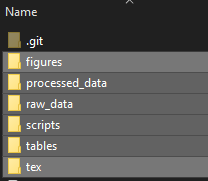
\includegraphics[width=0.3\linewidth]{img/folders} \end{center}

\hypertarget{first-r-script}{%
\subsection{First R script!}\label{first-r-script}}

Now that we have our folders created, let's now create paths to those folders with R. Let's start by creating a variable workingdir which we can define as the path to our main folder.

\begin{Shaded}
\begin{Highlighting}[]
\NormalTok{workingdir}\OtherTok{\textless{}{-}}\StringTok{"PATH\_TO\_YOUR\_WORKING\_DIR"}  \CommentTok{\# 1}
\end{Highlighting}
\end{Shaded}

Now we are going to create a script, let's save it as workingdir.R and place it in our main parent folder. We are then going to be using the path we defined above in this script to create paths to our other folders.

\begin{Shaded}
\begin{Highlighting}[]
\NormalTok{folder\_figures}\OtherTok{\textless{}{-}}\FunctionTok{paste0}\NormalTok{(workingdir, }\StringTok{"figures"}\NormalTok{)                }\CommentTok{\# 1}
\NormalTok{folder\_processed\_data}\OtherTok{\textless{}{-}}\FunctionTok{paste0}\NormalTok{(workingdir, }\StringTok{"processed\_data"}\NormalTok{)  }\CommentTok{\# 2}
\NormalTok{folder\_raw\_data}\OtherTok{\textless{}{-}}\FunctionTok{paste0}\NormalTok{(workingdir, }\StringTok{"raw\_data"}\NormalTok{)              }\CommentTok{\# 3}
\NormalTok{folder\_scripts}\OtherTok{\textless{}{-}}\FunctionTok{paste0}\NormalTok{(workingdir, }\StringTok{"scripts"}\NormalTok{)                }\CommentTok{\# 4}
\NormalTok{folder\_tables}\OtherTok{\textless{}{-}}\FunctionTok{paste0}\NormalTok{(workingdir, }\StringTok{"tables"}\NormalTok{)                  }\CommentTok{\# 5}
\NormalTok{folder\_tex}\OtherTok{\textless{}{-}}\FunctionTok{paste0}\NormalTok{(workingdir, }\StringTok{"tex"}\NormalTok{)                        }\CommentTok{\# 6}
\end{Highlighting}
\end{Shaded}

Now at the top of all other scripts we can have:

\begin{Shaded}
\begin{Highlighting}[]
\NormalTok{workingdir}\OtherTok{\textless{}{-}}\StringTok{"PATH\_TO\_YOUR\_WORKING\_DIR"}    \CommentTok{\# 1}
\FunctionTok{source}\NormalTok{(}\FunctionTok{paste0}\NormalTok{(workingdir, workingdir.r))  }\CommentTok{\# 2}
\end{Highlighting}
\end{Shaded}

Now all this says is we have a variable named workingdir that points to our main parent folder. We then have a script in which we define paths to all other folders. With this at the front of all of our scripts, we can easily reference them to create easier pathing for ourselves.

\hypertarget{downloading-within-r}{%
\section{Downloading within R}\label{downloading-within-r}}

We can use R to with a direct link to download. The first argument the download.file() command takes that we will use is the url of the xslx document and the second argument is the destination it will be saved. The last argument is basically telling R that the excel docs are not plain text. (Don't forget to have workingdir defined as we did in \href{https://jmwestenberg.github.io/courses/rcourse/intro/lesson1_03/}{Project Organization}

\begin{Shaded}
\begin{Highlighting}[]
\FunctionTok{download.file}\NormalTok{(}\StringTok{"https://www.bls.gov/lau/laucnty90.xlsx"}\NormalTok{,     }\CommentTok{\# 1}
  \FunctionTok{paste0}\NormalTok{(folder\_raw\_data, }\StringTok{"bls\_unemp\_90.xlsx"}\NormalTok{), }\AttributeTok{mode=}\StringTok{"wb"}\NormalTok{)  }\CommentTok{\# 2}
\end{Highlighting}
\end{Shaded}

\hypertarget{reading-in-data}{%
\section{Reading in Data}\label{reading-in-data}}

Before we read in this data to R, let's see what we are dealing with. Opening up the file in excel we can see there will be issues reading the file in.

\begin{center}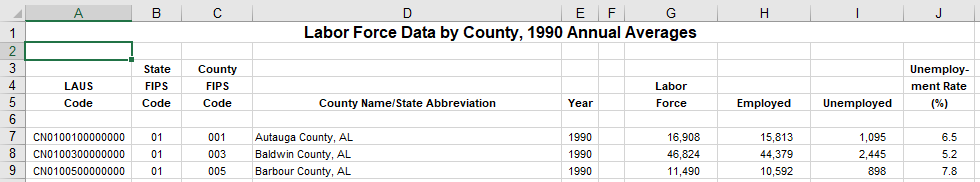
\includegraphics[width=0.8\linewidth]{img/data_head} \end{center}

We can notice that the first row has the file title spread across columns A:J. Variable names are spread across anywhere 1-3 rows. And lastly we have an empty column in F. The bright side is if we observe the other year's files, they all have this exact same structure. Hence we will able to use a loop eventually to clean them all instead of one at a time.

The main package we will be using is readxl, which is quite self explanatory. It is a package meant to help to read in excel docs. Let's try to open the file for 1990 we downloaded in R. We can do this through R Studio's functionality.

Within the ``Environment'' area of R Studio, click Import Dataset, then From Excel\ldots{}

\begin{center}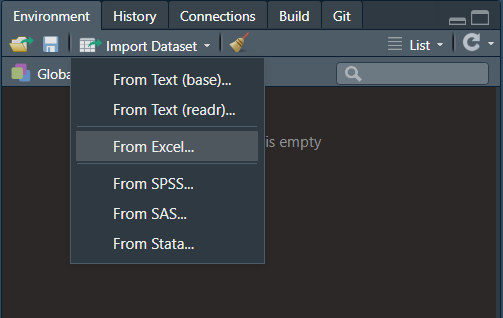
\includegraphics[width=0.4\linewidth]{img/import_fromexcel} \end{center}

There is definitely multiple ways to do this, as we can see from the options available. I first deselect ``First Row as Names'' (This option is very nice if your data is already in a precleaned form and your first row simply has your variable names.) I then begin to skip rows, 5 rows of skipping leads to the first row being the first row of data.

\begin{center}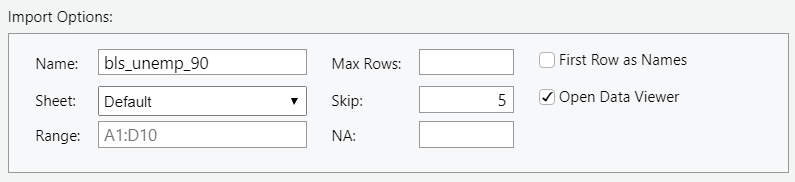
\includegraphics[width=0.7\linewidth]{img/import_fromexceloptions} \end{center}

Next we can handle column F that we noticed was blank. This is column 6 and stays consistent across all years (you can check this). Remembering our lessons from the Very Basics section we can subset this dataframe by removing column 6.

Hence we have something that will look like the following for our command for our script.

\begin{Shaded}
\begin{Highlighting}[]
\FunctionTok{require}\NormalTok{(readxl)                                                                           }\CommentTok{\# 1}
\NormalTok{workingdir}\OtherTok{\textless{}{-}}\StringTok{"C:/Users/weste/Documents/GitHub/r{-}introtodatascience/sample\_repo/"}           \CommentTok{\# 2}
\NormalTok{bls\_unemp\_90 }\OtherTok{\textless{}{-}} \FunctionTok{read\_excel}\NormalTok{(}\FunctionTok{paste0}\NormalTok{(folder\_raw\_data, }\StringTok{"/bls\_unemp\_90.xlsx"}\NormalTok{),                 }\CommentTok{\# 3}
                           \AttributeTok{col\_names=}\ConstantTok{FALSE}\NormalTok{, }\AttributeTok{skip=}\DecValTok{5}\NormalTok{)                                       }\CommentTok{\# 4}
\NormalTok{bls\_unemp\_90}\OtherTok{\textless{}{-}}\NormalTok{bls\_unemp\_90[,}\SpecialCharTok{{-}}\DecValTok{6}\NormalTok{]                                                           }\CommentTok{\# 5}
\FunctionTok{colnames}\NormalTok{(bls\_unemp\_90)}\OtherTok{\textless{}{-}}\FunctionTok{c}\NormalTok{(}\StringTok{"LAUS\_code"}\NormalTok{, }\StringTok{"State\_fips"}\NormalTok{, }\StringTok{"County\_fips"}\NormalTok{, }\StringTok{"County\_name"}\NormalTok{,        }\CommentTok{\# 6}
                          \StringTok{"Year"}\NormalTok{, }\StringTok{"Labor\_force"}\NormalTok{, }\StringTok{"Employed"}\NormalTok{, }\StringTok{"Unemployed"}\NormalTok{, }\StringTok{"Unemp\_rate"}\NormalTok{)  }\CommentTok{\# 7}
\end{Highlighting}
\end{Shaded}

Where the last line above we are giving our columns names based on the names we saw in the excel document.

We can then observe our data frame to ssee if it's fully cleaned. At first it seems so (I actually initially thought so). However when reading in the data, we grabbed 2 extra rows at the end of the file. Hence we have 2 rows at the end of our data frame that are NA's. Let's drop these two rows, to do this we can use a command is.na and prior to it include an ``!'', saying `not is.na'.

\begin{Shaded}
\begin{Highlighting}[]
\NormalTok{bls\_unemp\_90}\OtherTok{\textless{}{-}}\NormalTok{bls\_unemp\_90[}\SpecialCharTok{!}\FunctionTok{is.na}\NormalTok{(bls\_unemp\_90}\SpecialCharTok{$}\NormalTok{State\_fips),]  }\CommentTok{\# 1}
\end{Highlighting}
\end{Shaded}

\textbf{Here is a good place to pause if you want a challenge. You should have all the tools needed to write a loop to download all files from 1990-2019.}

\hypertarget{download-loop}{%
\section{Download Loop}\label{download-loop}}

In the next sections we will be using \href{https://www.bls.gov/lau/home.htm}{county level employment/labor force data from BLS} to learn more about working with actual data. We will be using the \textbf{Labor force data by county, yearly annual averages}. There is data from 1990-2019 (as of writing these notes). To start we are going to download this data and then read it into R.

We can use a loop to download/clean our data such as this:

\begin{Shaded}
\begin{Highlighting}[]
\FunctionTok{require}\NormalTok{(stringr)                                                                }\CommentTok{\# 1}
\FunctionTok{require}\NormalTok{(readxl)                                                                 }\CommentTok{\# 2}
\NormalTok{unemp\_data}\OtherTok{\textless{}{-}}\FunctionTok{data.frame}\NormalTok{()                                                        }\CommentTok{\# 3}
\NormalTok{years}\OtherTok{\textless{}{-}}\FunctionTok{c}\NormalTok{(}\DecValTok{90}\SpecialCharTok{:}\DecValTok{99}\NormalTok{, }\DecValTok{0}\SpecialCharTok{:}\DecValTok{19}\NormalTok{)                                                           }\CommentTok{\# 4}
\NormalTok{years}\OtherTok{\textless{}{-}}\FunctionTok{str\_pad}\NormalTok{(}\FunctionTok{as.character}\NormalTok{(years), }\DecValTok{2}\NormalTok{, }\StringTok{"left"}\NormalTok{, }\StringTok{"0"}\NormalTok{)                             }\CommentTok{\# 5}
\NormalTok{years\_l}\OtherTok{\textless{}{-}}\FunctionTok{length}\NormalTok{(years)                                                          }\CommentTok{\# 6}
\ControlFlowTok{for}\NormalTok{ (i }\ControlFlowTok{in} \DecValTok{1}\SpecialCharTok{:}\NormalTok{years\_l)\{                                                           }\CommentTok{\# 7}
\NormalTok{url}\OtherTok{\textless{}{-}}\FunctionTok{paste0}\NormalTok{(}\StringTok{"https://www.bls.gov/lau/laucnty"}\NormalTok{, years[i], }\StringTok{".xlsx"}\NormalTok{)               }\CommentTok{\# 8}
\NormalTok{destination}\OtherTok{\textless{}{-}}\FunctionTok{paste0}\NormalTok{(folder\_raw\_data, }\StringTok{"/bls\_unemp\_"}\NormalTok{, years[i], }\StringTok{".xlsx"}\NormalTok{)          }\CommentTok{\# 9}
\FunctionTok{download.file}\NormalTok{(url, destination, }\AttributeTok{mode=}\StringTok{"wb"}\NormalTok{)                                     }\CommentTok{\# 10}
\NormalTok{temp\_df }\OtherTok{\textless{}{-}} \FunctionTok{read\_excel}\NormalTok{(}\FunctionTok{paste0}\NormalTok{(folder\_raw\_data, }\StringTok{"/bls\_unemp\_"}\NormalTok{, years[i],         }\CommentTok{\# 11}
  \StringTok{".xlsx"}\NormalTok{),}\AttributeTok{col\_names=}\ConstantTok{FALSE}\NormalTok{, }\AttributeTok{skip=}\DecValTok{5}\NormalTok{)                                            }\CommentTok{\# 12}
\NormalTok{temp\_df}\OtherTok{\textless{}{-}}\NormalTok{temp\_df[,}\SpecialCharTok{{-}}\DecValTok{6}\NormalTok{]                                                          }\CommentTok{\# 13}
\FunctionTok{colnames}\NormalTok{(temp\_df)}\OtherTok{\textless{}{-}}\FunctionTok{c}\NormalTok{(}\StringTok{"LAUS\_code"}\NormalTok{, }\StringTok{"State\_fips"}\NormalTok{, }\StringTok{"County\_fips"}\NormalTok{, }\StringTok{"County\_name"}\NormalTok{,  }\CommentTok{\# 14}
  \StringTok{"Year"}\NormalTok{, }\StringTok{"Labor\_force"}\NormalTok{, }\StringTok{"Employed"}\NormalTok{, }\StringTok{"Unemployed"}\NormalTok{, }\StringTok{"Unemp\_rate"}\NormalTok{)               }\CommentTok{\# 15}
\NormalTok{temp\_df}\OtherTok{\textless{}{-}}\NormalTok{temp\_df[}\SpecialCharTok{!}\FunctionTok{is.na}\NormalTok{(temp\_df}\SpecialCharTok{$}\NormalTok{State\_fips),]                                  }\CommentTok{\# 16}
\NormalTok{unemp\_data}\OtherTok{\textless{}{-}}\FunctionTok{rbind}\NormalTok{(county\_data, temp\_df)                                        }\CommentTok{\# 17}
\NormalTok{\}                                                                              }\CommentTok{\# 18}
\NormalTok{filename}\OtherTok{\textless{}{-}}\FunctionTok{paste0}\NormalTok{(folder\_processed\_data, }\StringTok{"/unemp\_data.rda"}\NormalTok{)                     }\CommentTok{\# 19}
\FunctionTok{save}\NormalTok{(unemp\_data, }\AttributeTok{file=}\NormalTok{filename)                                                }\CommentTok{\# 20}
\end{Highlighting}
\end{Shaded}

To work through this first let's think what we are trying to achieve. The links for the downloads are all in the form of \href{https://www.bls.gov/lau/home.htm}{https://www.bls.gov/lau/laucntyZZ.xlsx}, where ZZ is two digits representing the year. These ZZ values run from ``90''to ``99'' for years 1990-1999 and ``00'' to ``19'' for years 2000-2019.

Let's work through the above code line by line:

\begin{itemize}
\tightlist
\item
  Lines \#1 \& \#2: load required packages.
\item
  Line \#3: Declare unemp\_data will be a data.frame. Right now it is empty, but we will add to it.
\item
  Line \#4: Define a vector with elements 90-99 and 0-19. (Which will correspond to the years that we will pull)
\item
  Line \#5 : We have a vector for years, however if we notice in the url names we need this vector to include a leading 0 in front of the single `character' digits (ie ``01'' instead of ``1''). But we don't want a leading 0 in front of the double `character' digits (ie We DON'T want ``090''). Go back to the \href{https://jmwestenberg.github.io/courses/rcourse/intro/lesson1_02/}{String Manipulation} section if you need to refresh on this.
\item
  Line \#6 : Calculate the length of years and save as years\_l
\item
  Line \#7 : See \href{https://jmwestenberg.github.io/courses/rcourse/intro/lesson1_02/}{String Manipulation} if defining the for loop does not make sense.
\item
  Line \#8 : We are creating the character string for the url for the download link. Since they all take the form of \url{https://www.bls.gov/lau/laucntyZZ.xlsx}, we can use one element of our years vector at a time. (See \href{https://jmwestenberg.github.io/courses/rcourse/intro/lesson1_02/}{String Manipulation} for explanation on paste0)
\item
  Line \#9 : This is of similar spirit to line \#4, but this is defining the path/filename of the excel file we will save.
\item
  Line \#10 : This line is just telling R to download the file at that url, save it to the defined location/name, and to read it as a non-raw text form. (see \href{https://jmwestenberg.github.io/courses/rcourse/intro/lesson1_04/}{Downloading/Reading Data} if unclear.)
\item
  Lines \#11-\#16: See \href{https://jmwestenberg.github.io/courses/rcourse/intro/lesson1_04/}{Downloading/Reading Data} for a direct explanation.
\item
  Line \#17: rbind appends data. Hence since all of our data has the same format and has a variable indicating the year, we can simply append.
\item
  Line \#19: Create the filepath (to our processed\_data folder) where we will save the file, what the file name and type is.
\item
  Line \#20: save the combined data to the location/name we defined above.
\end{itemize}

We now have our data cleaned and saved for our next lesson when we will start to work with it more!

\hypertarget{tidyverse}{%
\chapter{Tidyverse}\label{tidyverse}}

The goal of this Tidyverse section is to learn

\begin{itemize}
\tightlist
\item
  Subsetting Datasets
\item
  Merging Datasets
\item
  Summarizing
\item
  Plotting
\end{itemize}

In this section we will be continuing to be working with the BLS data we downloaded in the Introduction.

Tidyverse provides us with some useful tools for data manipulation and cleaning. I include examples and descriptions of the commands I have most frequently used.

\hypertarget{filtering-with-pipes}{%
\section{Filtering with Pipes}\label{filtering-with-pipes}}

\begin{Shaded}
\begin{Highlighting}[]
\NormalTok{indiana}\OtherTok{\textless{}{-}}                                    \CommentTok{\# 1  \# 1}
\NormalTok{    unemp\_data }\SpecialCharTok{\%\textgreater{}\%} \FunctionTok{filter}\NormalTok{(State\_fips}\SpecialCharTok{==}\StringTok{"18"}\NormalTok{)  }\CommentTok{\# 2  \# 2}
\end{Highlighting}
\end{Shaded}

What is going on in this line of code? Let's start with the second line. The operator \%\textgreater\% is called a pipe. This comes from a package called magittr which is included within tidyverse. Pipes are very handy for neatly writing longer sequences of code. Here we begin with a pretty simple example. We can think of pipes as saying ``then''. That is it takes the argument before it and uses it as input in the following command. Here we are using a filter command, so we are saying take our data.frame county\_data, then filter or ``give us'' the values where State\_fips is equal to ``18'' (this is fips code for Indiana. Go Hoosiers!). So in summary we are just filtering out indiana data and saving it as a new data frame (this is line 1). Note: this operation does NOT impact county\_data, the only way we `over write' a data frame is to explicitly tell it to. For example the following WOULD overwrite county\_data.

\begin{Shaded}
\begin{Highlighting}[]
\NormalTok{unemp\_data}\OtherTok{\textless{}{-}}\NormalTok{unemp\_data }\SpecialCharTok{\%\textgreater{}\%} \FunctionTok{filter}\NormalTok{(State\_fips}\SpecialCharTok{==}\StringTok{"18"}\NormalTok{)  }\CommentTok{\# 1  \# 1}
\end{Highlighting}
\end{Shaded}

\hypertarget{plotting-data}{%
\section{Plotting Data}\label{plotting-data}}

In this lesson we will be plotting the data gathered in previous lessons. ggplot2 is a very popular package for plotting and is now included as part of the tidyverse package. It allows us to make many different kinds of plots and customize them. As it is so popular there are many guides for it. \href{https://ggplot2.tidyverse.org/}{Tidyverse's website} summarizes some very useful resources.

As ggplot2 has so many options, we will just be barely skimming the surface in this introduction. Let's start with a minimal command. First let's load in ggplot2 filter our data down into just Indiana.

\begin{Shaded}
\begin{Highlighting}[]
\FunctionTok{library}\NormalTok{(ggplot2)                                    }\CommentTok{\# 1  \# 1}
                                                    \CommentTok{\# 2  \# 2}
\NormalTok{indiana }\OtherTok{\textless{}{-}}\NormalTok{ unemp\_data }\SpecialCharTok{\%\textgreater{}\%} \FunctionTok{filter}\NormalTok{(State\_fips}\SpecialCharTok{==}\StringTok{"18"}\NormalTok{)  }\CommentTok{\# 3  \# 3}
\end{Highlighting}
\end{Shaded}

\begin{Shaded}
\begin{Highlighting}[]
\FunctionTok{ggplot}\NormalTok{(}\AttributeTok{data=}\NormalTok{indiana, }\FunctionTok{aes}\NormalTok{(}\AttributeTok{x=}\NormalTok{Year, }\AttributeTok{y=}\NormalTok{Unemp\_rate,   }\CommentTok{\# 1  \# 1}
    \AttributeTok{colour=}\NormalTok{County\_fips, }\AttributeTok{group=}\NormalTok{County\_fips))}\SpecialCharTok{+}     \CommentTok{\# 2  \# 2}
  \FunctionTok{geom\_line}\NormalTok{()                                    }\CommentTok{\# 3  \# 3}
\end{Highlighting}
\end{Shaded}

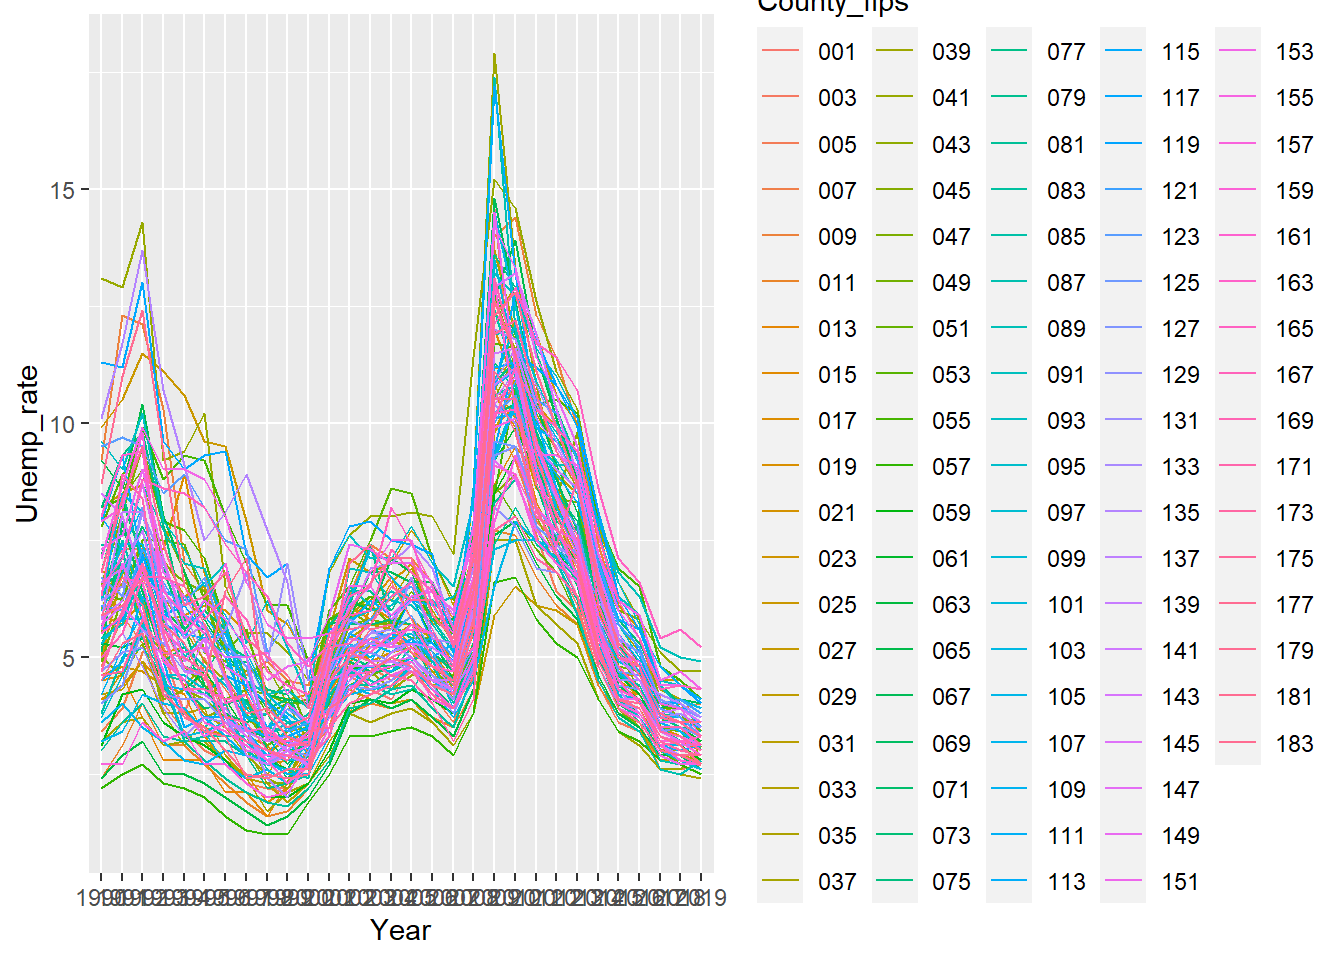
\includegraphics{bookdown-demo_files/figure-latex/unnamed-chunk-37-1.pdf}

\begin{itemize}
\tightlist
\item
  Line \#1: Tells ggplot we will be using the data.frame indiana. aes is short for aesthetics. This is where we tell ggplot how to map our data into the plots. Here I want ggplot to plot Year on the x-axis, Unemp\_rate on the y-axis.
\item
  Line \#2: A continuation of the aesthetic mapping, his line is saying plot separately for each County\_fips separately, giving them a different color.
\item
  Line \#3: Tells ggplot to plot the data as lines.
\end{itemize}

First thing after this plot, the legend is excessive. Let's just suppress it for now. To do this we can define the legend.position in theme as none. The theme command allows for a lot of customization with the plot. If you want to see all options \href{https://ggplot2.tidyverse.org/reference/theme.html}{click here.} Let's also change the thickness of the lines, we can do this with the alpha argument.

\begin{Shaded}
\begin{Highlighting}[]
\FunctionTok{ggplot}\NormalTok{(}\AttributeTok{data=}\NormalTok{indiana, }\FunctionTok{aes}\NormalTok{(}\AttributeTok{x=}\NormalTok{Year, }\AttributeTok{y=}\NormalTok{Unemp\_rate,   }\CommentTok{\# 1  \# 1}
    \AttributeTok{colour=}\NormalTok{County\_fips, }\AttributeTok{group=}\NormalTok{County\_fips))}\SpecialCharTok{+}     \CommentTok{\# 2  \# 2}
  \FunctionTok{geom\_line}\NormalTok{(}\AttributeTok{size=}\FloatTok{0.3}\NormalTok{)}\SpecialCharTok{+}                           \CommentTok{\# 3  \# 3}
  \FunctionTok{theme}\NormalTok{(}\AttributeTok{legend.position=}\StringTok{"none"}\NormalTok{)                  }\CommentTok{\# 4  \# 4}
\end{Highlighting}
\end{Shaded}

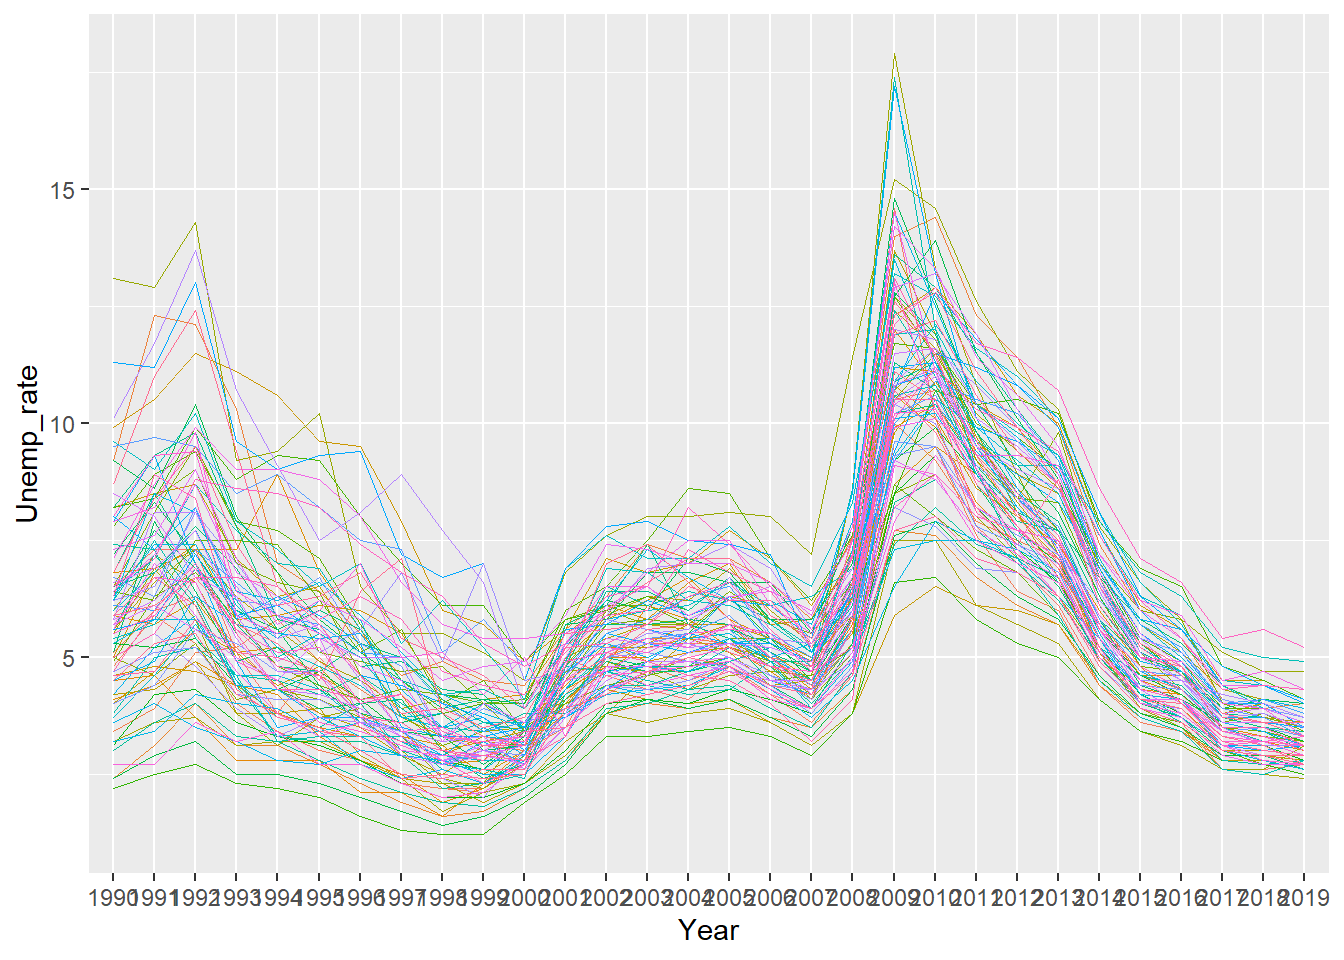
\includegraphics{bookdown-demo_files/figure-latex/unnamed-chunk-38-1.pdf}

This already is looking a lot better. But can we do something about the labels on the x axis, they are overlaying on each other. We could make the text smaller but then it would be difficult to see, so let's just rotate them. Also let's make the y-axis name a bit more meaningful.

\begin{Shaded}
\begin{Highlighting}[]
\FunctionTok{ggplot}\NormalTok{(}\AttributeTok{data=}\NormalTok{indiana, }\FunctionTok{aes}\NormalTok{(}\AttributeTok{x=}\NormalTok{Year, }\AttributeTok{y=}\NormalTok{Unemp\_rate,   }\CommentTok{\# 1  \# 1}
    \AttributeTok{colour=}\NormalTok{County\_fips, }\AttributeTok{group=}\NormalTok{County\_fips))}\SpecialCharTok{+}     \CommentTok{\# 2  \# 2}
  \FunctionTok{geom\_line}\NormalTok{(}\AttributeTok{size=}\FloatTok{0.3}\NormalTok{)}\SpecialCharTok{+}                           \CommentTok{\# 3  \# 3}
  \FunctionTok{theme}\NormalTok{(}\AttributeTok{legend.position=}\StringTok{"none"}\NormalTok{,                  }\CommentTok{\# 4  \# 4}
    \AttributeTok{axis.text.x=}\FunctionTok{element\_text}\NormalTok{(}\AttributeTok{angle=}\DecValTok{45}\NormalTok{)) }\SpecialCharTok{+}        \CommentTok{\# 5  \# 5}
  \FunctionTok{ylab}\NormalTok{(}\StringTok{\textquotesingle{}Indiana Unemployment Rate by County\textquotesingle{}}\NormalTok{)    }\CommentTok{\# 6  \# 6}
\end{Highlighting}
\end{Shaded}

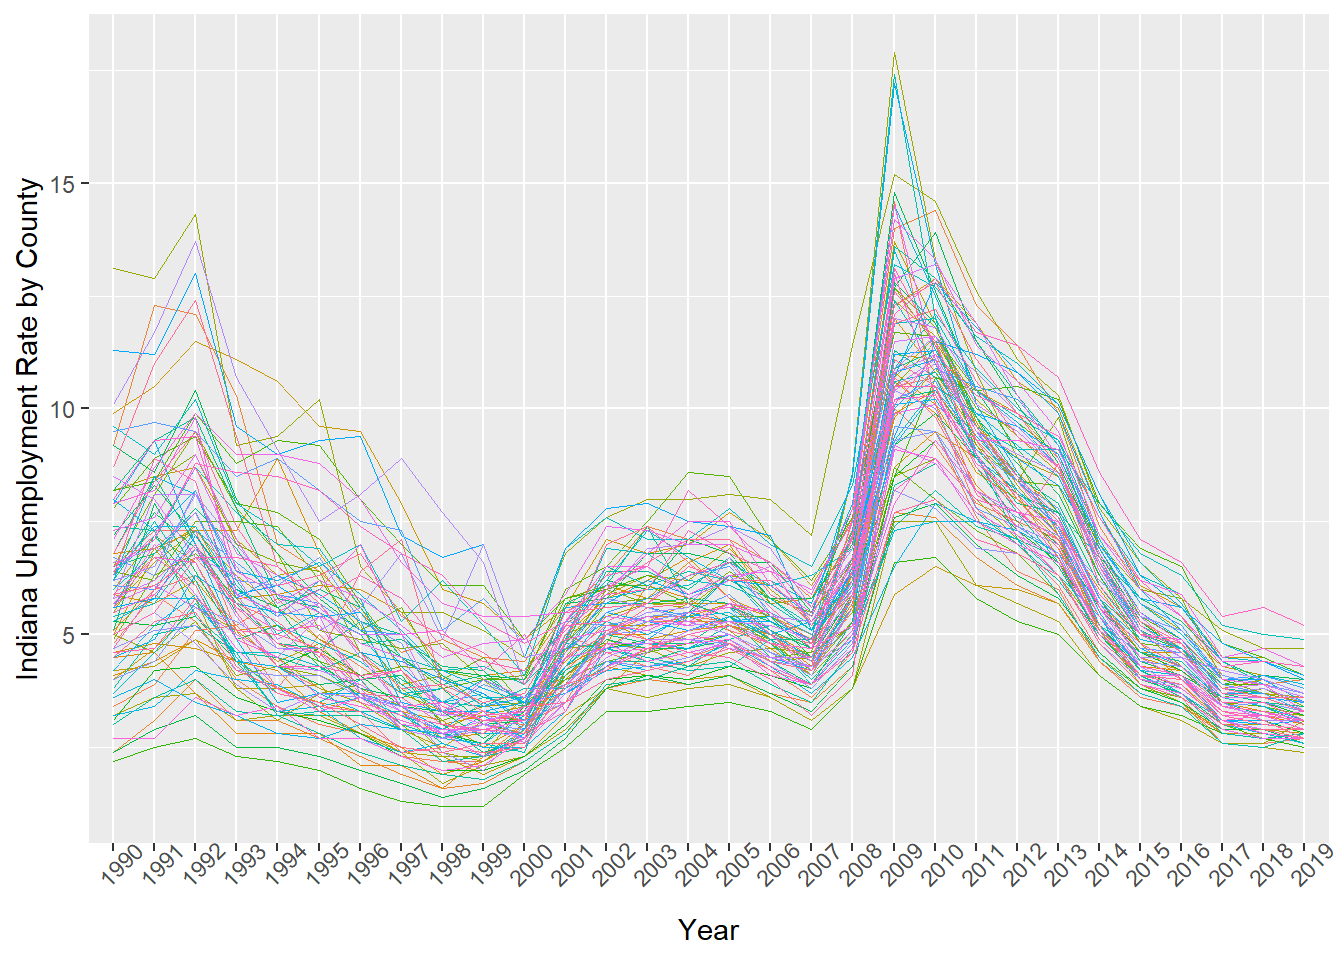
\includegraphics{bookdown-demo_files/figure-latex/unnamed-chunk-39-1.pdf}

Now we're getting somewhere! But what if we want to emphasize the county Bloomington is in, Monroe County?

\begin{Shaded}
\begin{Highlighting}[]
\NormalTok{monroecty}\OtherTok{\textless{}{-}}\NormalTok{indiana }\SpecialCharTok{\%\textgreater{}\%} \FunctionTok{filter}\NormalTok{(County\_fips}\SpecialCharTok{==}\StringTok{"105"}\NormalTok{)       }\CommentTok{\# 1   \# 1}
                                                        \CommentTok{\# 2   \# 2}
\FunctionTok{ggplot}\NormalTok{(}\AttributeTok{data=}\NormalTok{indiana, }\FunctionTok{aes}\NormalTok{(}\AttributeTok{x=}\NormalTok{Year, }\AttributeTok{y=}\NormalTok{Unemp\_rate,          }\CommentTok{\# 3   \# 3}
    \AttributeTok{colour=}\NormalTok{County\_fips, }\AttributeTok{group=}\NormalTok{County\_fips))}\SpecialCharTok{+}            \CommentTok{\# 4   \# 4}
  \FunctionTok{geom\_line}\NormalTok{(}\AttributeTok{size=}\FloatTok{0.3}\NormalTok{)}\SpecialCharTok{+}                                  \CommentTok{\# 5   \# 5}
  \FunctionTok{geom\_line}\NormalTok{(}\AttributeTok{data=}\NormalTok{monroecty, }\FunctionTok{aes}\NormalTok{(}\AttributeTok{x=}\NormalTok{Year, }\AttributeTok{y=}\NormalTok{Unemp\_rate,   }\CommentTok{\# 6   \# 6}
    \AttributeTok{colour=}\NormalTok{County\_fips, }\AttributeTok{group=}\DecValTok{1}\NormalTok{),                       }\CommentTok{\# 7   \# 7}
    \AttributeTok{size=}\FloatTok{0.6}\NormalTok{, }\AttributeTok{colour=}\StringTok{\textquotesingle{}black\textquotesingle{}}\NormalTok{) }\SpecialCharTok{+}                         \CommentTok{\# 8   \# 8}
  \FunctionTok{theme}\NormalTok{(}\AttributeTok{legend.position=}\StringTok{"none"}\NormalTok{,                         }\CommentTok{\# 9   \# 9}
    \AttributeTok{axis.text.x=}\FunctionTok{element\_text}\NormalTok{(}\AttributeTok{angle=}\DecValTok{45}\NormalTok{)) }\SpecialCharTok{+}              \CommentTok{\# 10  \# 10}
  \FunctionTok{ylab}\NormalTok{(}\StringTok{\textquotesingle{}Indiana Unemployment Rate by County\textquotesingle{}}\NormalTok{)          }\CommentTok{\# 11  \# 11}
\end{Highlighting}
\end{Shaded}

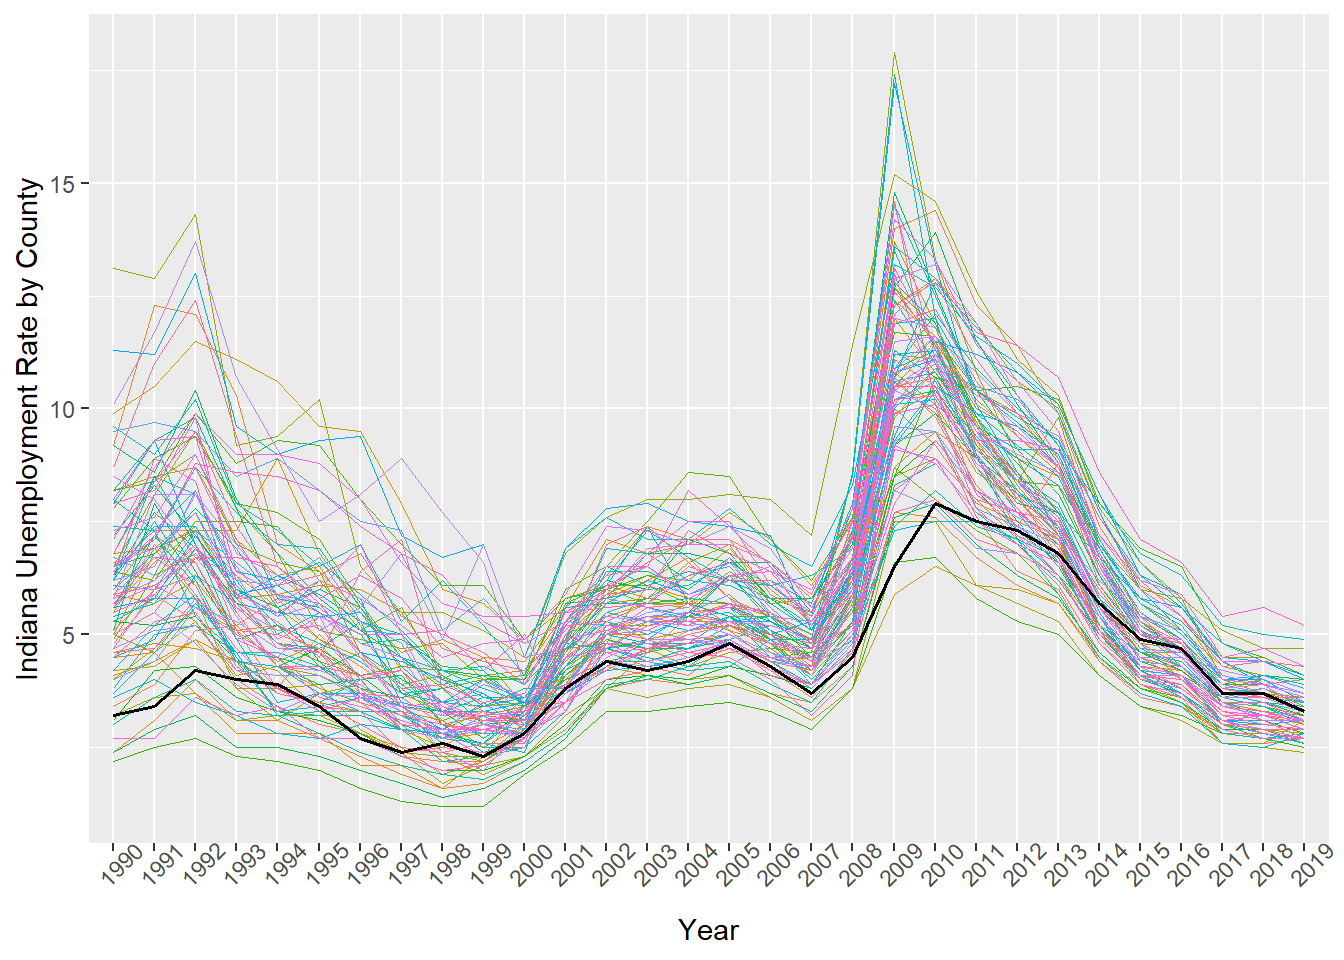
\includegraphics{bookdown-demo_files/figure-latex/unnamed-chunk-40-1.pdf}

We can make the black line for Monroe County `pop' a bit more too. Let's change the opacity of the other counties lines. To do this we can set a value, alpha. This takes values 0 to 1 where smaller values are more transparent.

\begin{Shaded}
\begin{Highlighting}[]
\FunctionTok{ggplot}\NormalTok{(}\AttributeTok{data=}\NormalTok{indiana, }\FunctionTok{aes}\NormalTok{(}\AttributeTok{x=}\NormalTok{Year, }\AttributeTok{y=}\NormalTok{Unemp\_rate,          }\CommentTok{\# 1  \# 1}
    \AttributeTok{colour=}\NormalTok{County\_fips, }\AttributeTok{group=}\NormalTok{County\_fips))}\SpecialCharTok{+}            \CommentTok{\# 2  \# 2}
  \FunctionTok{geom\_line}\NormalTok{(}\AttributeTok{size=}\FloatTok{0.3}\NormalTok{, }\AttributeTok{alpha=}\FloatTok{0.5}\NormalTok{)}\SpecialCharTok{+}                       \CommentTok{\# 3  \# 3}
  \FunctionTok{geom\_line}\NormalTok{(}\AttributeTok{data=}\NormalTok{monroecty, }\FunctionTok{aes}\NormalTok{(}\AttributeTok{x=}\NormalTok{Year, }\AttributeTok{y=}\NormalTok{Unemp\_rate,   }\CommentTok{\# 4  \# 4}
    \AttributeTok{colour=}\NormalTok{County\_fips, }\AttributeTok{group=}\DecValTok{1}\NormalTok{),                       }\CommentTok{\# 5  \# 5}
    \AttributeTok{size=}\FloatTok{0.6}\NormalTok{, }\AttributeTok{colour=}\StringTok{\textquotesingle{}black\textquotesingle{}}\NormalTok{) }\SpecialCharTok{+}                         \CommentTok{\# 6  \# 6}
  \FunctionTok{theme}\NormalTok{(}\AttributeTok{legend.position=}\StringTok{"none"}\NormalTok{,                         }\CommentTok{\# 7  \# 7}
    \AttributeTok{axis.text.x=}\FunctionTok{element\_text}\NormalTok{(}\AttributeTok{angle=}\DecValTok{45}\NormalTok{)) }\SpecialCharTok{+}               \CommentTok{\# 8  \# 8}
  \FunctionTok{ylab}\NormalTok{(}\StringTok{\textquotesingle{}Indiana Unemployment Rate by County\textquotesingle{}}\NormalTok{)           }\CommentTok{\# 9  \# 9}
\end{Highlighting}
\end{Shaded}

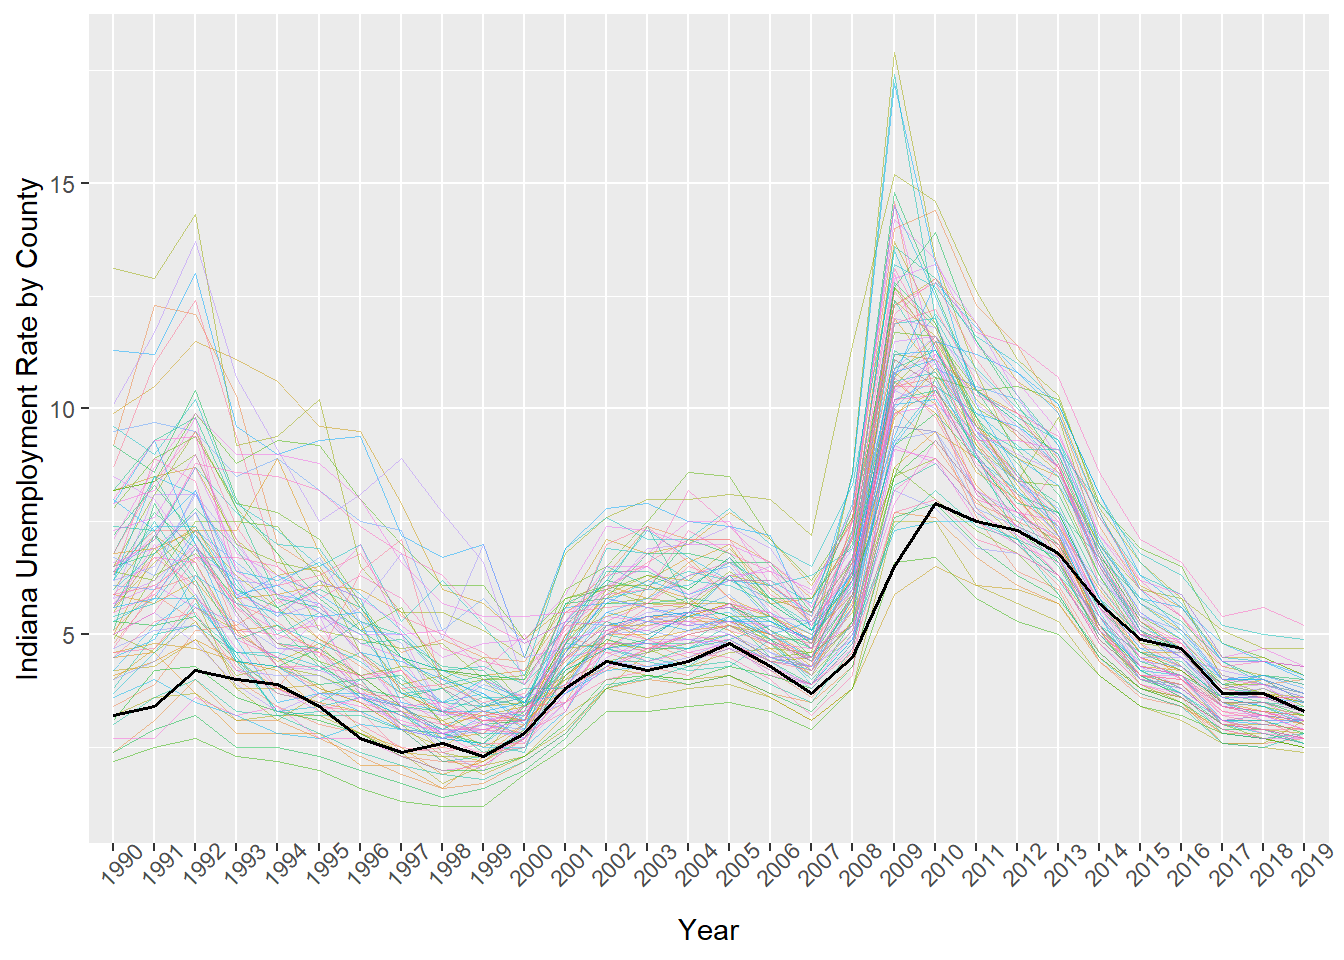
\includegraphics{bookdown-demo_files/figure-latex/unnamed-chunk-41-1.pdf}

\hypertarget{scatter-plot-geom_point}{%
\subsection{Scatter plot (geom\_point)}\label{scatter-plot-geom_point}}

What if we want points to insteaed of lines for each year?

\begin{Shaded}
\begin{Highlighting}[]
\FunctionTok{ggplot}\NormalTok{(}\AttributeTok{data=}\NormalTok{indiana, }\FunctionTok{aes}\NormalTok{(}\AttributeTok{x=}\NormalTok{Year, }\AttributeTok{y=}\NormalTok{Unemp\_rate,   }\CommentTok{\# 1  \# 1}
  \AttributeTok{colour=}\NormalTok{County\_fips, }\AttributeTok{group=}\NormalTok{County\_fips))}\SpecialCharTok{+}       \CommentTok{\# 2  \# 2}
  \FunctionTok{geom\_point}\NormalTok{()                                   }\CommentTok{\# 3  \# 3}
\end{Highlighting}
\end{Shaded}

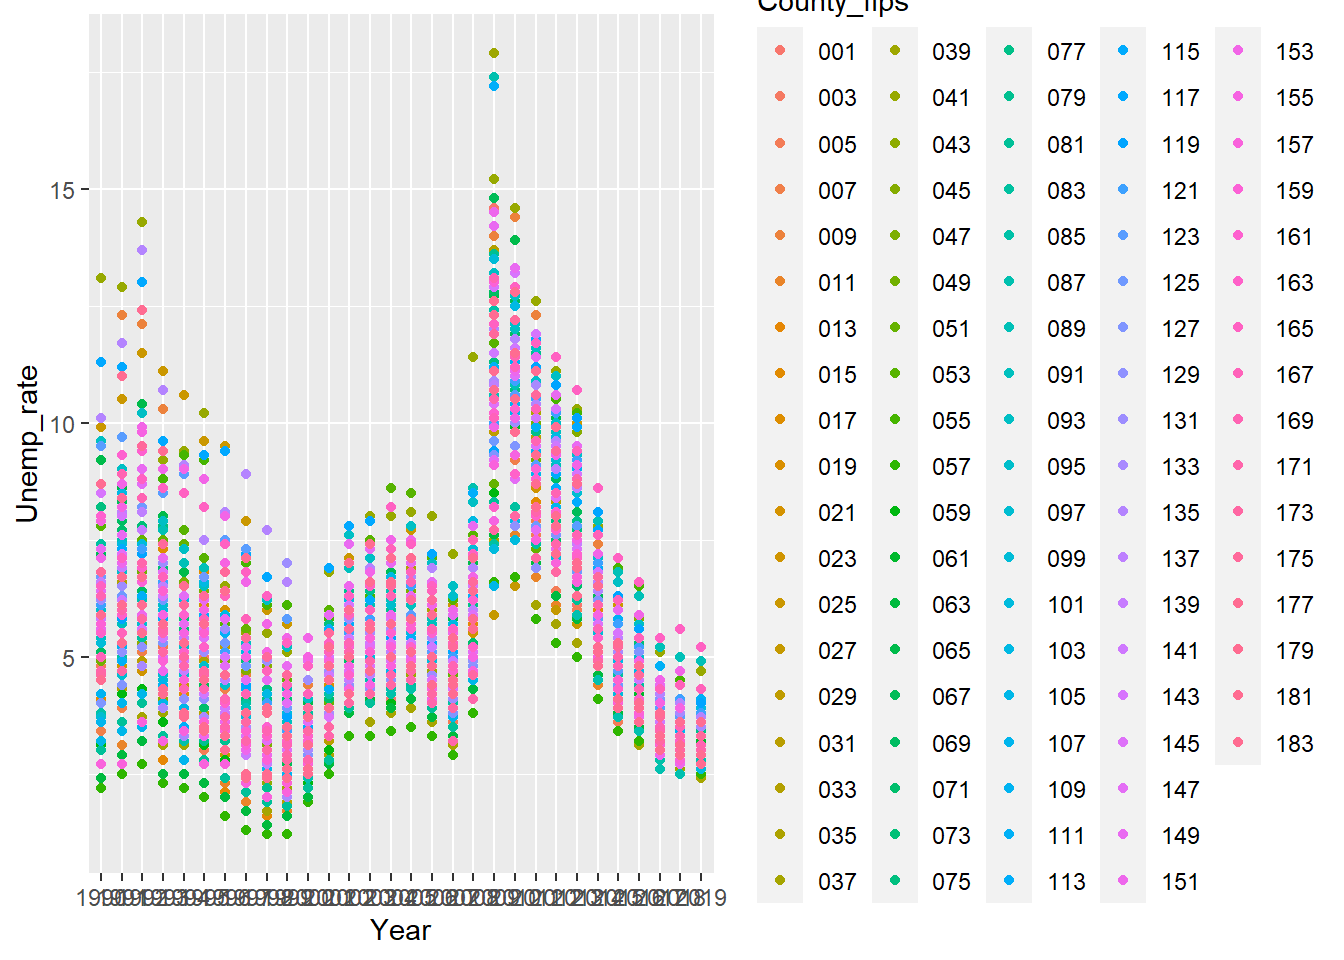
\includegraphics{bookdown-demo_files/figure-latex/unnamed-chunk-42-1.pdf}

\hypertarget{manipulating-within-groups}{%
\section{Manipulating within Groups}\label{manipulating-within-groups}}

Our next chunk of code gets a bit more complex, let's take it peice by peice though.

\begin{Shaded}
\begin{Highlighting}[]
\NormalTok{  indiana }\SpecialCharTok{\%\textgreater{}\%} \FunctionTok{group\_by}\NormalTok{(Year) }\SpecialCharTok{\%\textgreater{}\%}          \CommentTok{\# 1  \# 1}
    \FunctionTok{summarise}\NormalTok{(}\AttributeTok{Average=}\FunctionTok{mean}\NormalTok{(Labor\_force))  }\CommentTok{\# 2  \# 2}
\end{Highlighting}
\end{Shaded}

Let's again take it from the end and work our ways backwards through it. The 3rd line above is calculating a new variable within a group that is called `Average'. The group (line 2) that we are calculating within is each Year for our Indiana data.frame. That is this snippet of code will give us one value back for each year, the average Labor Force level across Indiana's counties.

\begin{tabular}{l|r}
\hline
Year & Average\\
\hline
1990 & 30593.65\\
\hline
1991 & 30357.00\\
\hline
1992 & 31058.60\\
\hline
1993 & 32046.84\\
\hline
1994 & 33308.01\\
\hline
1995 & 34078.00\\
\hline
1996 & 33800.80\\
\hline
1997 & 33919.72\\
\hline
1998 & 33947.47\\
\hline
1999 & 33965.91\\
\hline
2000 & 33982.50\\
\hline
2001 & 34140.32\\
\hline
2002 & 34469.34\\
\hline
2003 & 34597.76\\
\hline
2004 & 34432.72\\
\hline
2005 & 34841.75\\
\hline
2006 & 35164.35\\
\hline
2007 & 34866.21\\
\hline
2008 & 35131.49\\
\hline
2009 & 34717.45\\
\hline
2010 & 34512.97\\
\hline
2011 & 34586.91\\
\hline
2012 & 34454.88\\
\hline
2013 & 34656.59\\
\hline
2014 & 35052.00\\
\hline
2015 & 35508.30\\
\hline
2016 & 36178.11\\
\hline
2017 & 36243.96\\
\hline
2018 & 36756.59\\
\hline
2019 & 36819.25\\
\hline
\end{tabular}

This group\_by command paired with summarise is quite useful. For example going back to our original data.frame, county\_data. Suppose we wanted to do what we just did but for all states. That is calculate within each state and year combination. With the group\_by command this is quite simple! (I print the first 100 lines of output below)

\begin{Shaded}
\begin{Highlighting}[]
\NormalTok{unemp\_data }\SpecialCharTok{\%\textgreater{}\%}                          \CommentTok{\# 1  \# 1}
  \FunctionTok{group\_by}\NormalTok{(Year, State\_fips) }\SpecialCharTok{\%\textgreater{}\%}        \CommentTok{\# 2  \# 2}
  \FunctionTok{summarise}\NormalTok{(}\AttributeTok{Average=}\FunctionTok{mean}\NormalTok{(Labor\_force))  }\CommentTok{\# 3  \# 3}
\end{Highlighting}
\end{Shaded}

\begin{verbatim}
## `summarise()` has grouped output by 'Year'. You can override using the `.groups` argument.
\end{verbatim}

\begin{tabular}{l|l|r}
\hline
Year & State\_fips & Average\\
\hline
1990 & 01 & 28468.343\\
\hline
1990 & 02 & 10323.923\\
\hline
1990 & 04 & 119079.067\\
\hline
1990 & 05 & 15091.147\\
\hline
1990 & 06 & 261007.414\\
\hline
1990 & 08 & 27557.641\\
\hline
1990 & 09 & 227471.000\\
\hline
1990 & 10 & 120074.667\\
\hline
1990 & 11 & 328924.000\\
\hline
1990 & 12 & 96480.269\\
\hline
1990 & 13 & 20653.579\\
\hline
1990 & 15 & 137730.500\\
\hline
1990 & 16 & 11193.045\\
\hline
1990 & 17 & 58304.049\\
\hline
1990 & 18 & 30593.652\\
\hline
1990 & 19 & 14664.212\\
\hline
1990 & 20 & 12119.305\\
\hline
1990 & 21 & 14619.667\\
\hline
1990 & 22 & 29216.547\\
\hline
1990 & 23 & 39563.625\\
\hline
1990 & 24 & 107919.000\\
\hline
1990 & 25 & 229027.357\\
\hline
1990 & 26 & 55509.072\\
\hline
1990 & 27 & 27573.690\\
\hline
1990 & 28 & 14438.854\\
\hline
1990 & 29 & 22737.852\\
\hline
1990 & 30 & 7198.929\\
\hline
1990 & 31 & 8871.215\\
\hline
1990 & 32 & 39407.176\\
\hline
1990 & 33 & 62009.100\\
\hline
1990 & 34 & 193117.000\\
\hline
1990 & 35 & 21630.061\\
\hline
1990 & 36 & 142149.565\\
\hline
1990 & 37 & 34765.130\\
\hline
1990 & 38 & 5985.226\\
\hline
1990 & 39 & 61586.670\\
\hline
1990 & 40 & 19786.338\\
\hline
1990 & 41 & 41408.833\\
\hline
1990 & 42 & 86992.045\\
\hline
1990 & 44 & 105072.600\\
\hline
1990 & 45 & 37903.326\\
\hline
1990 & 46 & 5260.303\\
\hline
1990 & 47 & 25207.768\\
\hline
1990 & 48 & 33932.858\\
\hline
1990 & 49 & 28352.138\\
\hline
1990 & 50 & 21768.214\\
\hline
1990 & 51 & 24452.541\\
\hline
1990 & 53 & 64751.974\\
\hline
1990 & 54 & 13857.600\\
\hline
1990 & 55 & 35970.542\\
\hline
1990 & 56 & 10259.348\\
\hline
1990 & 72 & 14517.090\\
\hline
1991 & 01 & 28665.134\\
\hline
1991 & 02 & 10626.000\\
\hline
1991 & 04 & 120334.200\\
\hline
1991 & 05 & 15060.213\\
\hline
1991 & 06 & 260801.552\\
\hline
1991 & 08 & 28035.766\\
\hline
1991 & 09 & 230137.750\\
\hline
1991 & 10 & 120571.333\\
\hline
1991 & 11 & 321433.000\\
\hline
1991 & 12 & 97499.104\\
\hline
1991 & 13 & 20619.044\\
\hline
1991 & 15 & 142897.250\\
\hline
1991 & 16 & 11547.432\\
\hline
1991 & 17 & 58277.431\\
\hline
1991 & 18 & 30357.000\\
\hline
1991 & 19 & 14896.960\\
\hline
1991 & 20 & 12190.105\\
\hline
1991 & 21 & 14689.508\\
\hline
1991 & 22 & 29804.094\\
\hline
1991 & 23 & 40318.625\\
\hline
1991 & 24 & 109023.333\\
\hline
1991 & 25 & 228211.357\\
\hline
1991 & 26 & 55369.482\\
\hline
1991 & 27 & 27903.586\\
\hline
1991 & 28 & 14439.512\\
\hline
1991 & 29 & 23000.835\\
\hline
1991 & 30 & 7247.179\\
\hline
1991 & 31 & 8992.527\\
\hline
1991 & 32 & 41338.118\\
\hline
1991 & 33 & 61429.900\\
\hline
1991 & 34 & 193610.571\\
\hline
1991 & 35 & 21974.485\\
\hline
1991 & 36 & 140985.613\\
\hline
1991 & 37 & 35380.200\\
\hline
1991 & 38 & 5947.509\\
\hline
1991 & 39 & 61726.409\\
\hline
1991 & 40 & 19575.922\\
\hline
1991 & 41 & 42135.556\\
\hline
1991 & 42 & 87390.030\\
\hline
1991 & 44 & 103603.400\\
\hline
1991 & 45 & 38234.348\\
\hline
1991 & 46 & 5303.182\\
\hline
1991 & 47 & 25407.611\\
\hline
1991 & 48 & 34512.854\\
\hline
1991 & 49 & 29390.414\\
\hline
1991 & 50 & 21683.857\\
\hline
1991 & 51 & 25107.677\\
\hline
1991 & 53 & 65281.667\\
\hline
\end{tabular}

Average is just one statistic we may want to calculate, how about percentiles, minimum, maximum, standard deviation. our summarise command will accept more than one argument, we just have to separate by a comma. Let's also save this as a new data.frame for use in future lessons.

\begin{Shaded}
\begin{Highlighting}[]
\NormalTok{indiana\_laborforce}\OtherTok{\textless{}{-}}                       \CommentTok{\# 1   \# 1}
\NormalTok{  indiana }\SpecialCharTok{\%\textgreater{}\%} \FunctionTok{group\_by}\NormalTok{(Year) }\SpecialCharTok{\%\textgreater{}\%}           \CommentTok{\# 2   \# 2}
  \FunctionTok{summarise}\NormalTok{(}\AttributeTok{Min=}\FunctionTok{min}\NormalTok{(Labor\_force),          }\CommentTok{\# 3   \# 3}
    \AttributeTok{p10th=}\FunctionTok{quantile}\NormalTok{(Labor\_force, }\FunctionTok{c}\NormalTok{(}\FloatTok{0.1}\NormalTok{)),   }\CommentTok{\# 4   \# 4}
    \AttributeTok{p25th=}\FunctionTok{quantile}\NormalTok{(Labor\_force, }\FunctionTok{c}\NormalTok{(}\FloatTok{0.25}\NormalTok{)),  }\CommentTok{\# 5   \# 5}
    \AttributeTok{p50th=}\FunctionTok{quantile}\NormalTok{(Labor\_force, }\FunctionTok{c}\NormalTok{(}\FloatTok{0.5}\NormalTok{)),   }\CommentTok{\# 6   \# 6}
    \AttributeTok{p75th=}\FunctionTok{quantile}\NormalTok{(Labor\_force, }\FunctionTok{c}\NormalTok{(}\FloatTok{0.75}\NormalTok{)),  }\CommentTok{\# 7   \# 7}
    \AttributeTok{p90th=}\FunctionTok{quantile}\NormalTok{(Labor\_force, }\FunctionTok{c}\NormalTok{(}\FloatTok{0.9}\NormalTok{)),   }\CommentTok{\# 8   \# 8}
    \AttributeTok{Max=}\FunctionTok{max}\NormalTok{(Labor\_force),                  }\CommentTok{\# 9   \# 9}
    \AttributeTok{Average=}\FunctionTok{mean}\NormalTok{(Labor\_force),            }\CommentTok{\# 10  \# 10}
    \AttributeTok{StDev=}\FunctionTok{sd}\NormalTok{(Labor\_force))                }\CommentTok{\# 11  \# 11}
\end{Highlighting}
\end{Shaded}

\begin{tabular}{l|r|r|r|r|r|r|r|r|r}
\hline
Year & Min & p10th & p25th & p50th & p75th & p90th & Max & Average & StDev\\
\hline
1990 & 2629 & 6639.3 & 9617.50 & 14858.5 & 30089.50 & 60784.5 & 424053 & 30593.65 & 52989.19\\
\hline
1991 & 2541 & 6380.5 & 9480.00 & 14713.0 & 30131.00 & 62309.9 & 421789 & 30357.00 & 52670.08\\
\hline
1992 & 2550 & 6284.2 & 9615.50 & 15169.5 & 31117.00 & 63623.2 & 429239 & 31058.60 & 53551.02\\
\hline
1993 & 2607 & 6200.6 & 10037.75 & 15652.5 & 32034.75 & 64549.9 & 438377 & 32046.84 & 54683.97\\
\hline
1994 & 2681 & 6453.1 & 10480.50 & 16472.0 & 33808.25 & 66506.3 & 453457 & 33308.01 & 56427.35\\
\hline
1995 & 2714 & 6543.2 & 10994.75 & 16648.5 & 34588.00 & 67364.5 & 459603 & 34078.00 & 57219.27\\
\hline
1996 & 2724 & 6522.6 & 10827.50 & 16551.0 & 34597.25 & 66487.5 & 453728 & 33800.80 & 56670.37\\
\hline
1997 & 2698 & 6585.3 & 10966.00 & 16671.5 & 34786.50 & 66195.3 & 453928 & 33919.72 & 56870.28\\
\hline
1998 & 2701 & 6629.7 & 11008.75 & 16660.0 & 34150.50 & 65887.6 & 452412 & 33947.47 & 56827.82\\
\hline
1999 & 2691 & 6496.7 & 10986.75 & 16958.5 & 33968.50 & 65196.0 & 448732 & 33965.91 & 56434.89\\
\hline
2000 & 2985 & 7053.5 & 10816.50 & 16984.5 & 34996.50 & 63718.6 & 455135 & 33982.50 & 56818.02\\
\hline
2001 & 2982 & 7085.7 & 10709.00 & 17127.5 & 34674.75 & 64832.0 & 459505 & 34140.32 & 57318.59\\
\hline
2002 & 3051 & 7040.7 & 10802.75 & 17244.5 & 34974.75 & 66572.3 & 462330 & 34469.34 & 57807.67\\
\hline
2003 & 3092 & 6941.0 & 10709.50 & 17199.0 & 34514.75 & 67751.5 & 464331 & 34597.76 & 58056.22\\
\hline
2004 & 3109 & 6815.2 & 10547.00 & 17083.5 & 33431.50 & 68476.2 & 459140 & 34432.72 & 57583.09\\
\hline
2005 & 3152 & 7075.8 & 10702.75 & 17357.5 & 33606.00 & 69985.6 & 459492 & 34841.75 & 57925.42\\
\hline
2006 & 3107 & 6883.1 & 10620.50 & 17326.5 & 34554.50 & 72792.0 & 461468 & 35164.35 & 58484.53\\
\hline
2007 & 3026 & 6816.7 & 10447.50 & 16881.0 & 34304.50 & 73128.1 & 460046 & 34866.21 & 58342.88\\
\hline
2008 & 3044 & 6816.2 & 10488.00 & 16673.5 & 34065.50 & 75072.0 & 463200 & 35131.49 & 58819.13\\
\hline
2009 & 3088 & 6758.4 & 10434.25 & 16452.0 & 33700.25 & 74434.1 & 457524 & 34717.45 & 58083.80\\
\hline
2010 & 3263 & 6440.5 & 10308.00 & 16622.0 & 33921.75 & 74406.0 & 452836 & 34512.97 & 57806.16\\
\hline
2011 & 3210 & 6459.9 & 10184.25 & 16630.5 & 33804.00 & 75620.5 & 456011 & 34586.91 & 58199.53\\
\hline
2012 & 3181 & 6336.2 & 10058.50 & 16453.0 & 32924.00 & 76458.0 & 458377 & 34454.88 & 58388.80\\
\hline
2013 & 3165 & 6325.9 & 9900.50 & 16289.5 & 33053.00 & 78149.5 & 463346 & 34656.59 & 58983.65\\
\hline
2014 & 3216 & 6401.2 & 9851.50 & 16524.0 & 33215.50 & 80113.3 & 467169 & 35052.00 & 59579.47\\
\hline
2015 & 3178 & 6341.8 & 9924.75 & 16908.0 & 33960.00 & 82327.7 & 472330 & 35508.30 & 60275.44\\
\hline
2016 & 3226 & 6444.8 & 9930.50 & 17093.5 & 35149.00 & 85223.0 & 481434 & 36178.11 & 61517.07\\
\hline
2017 & 3153 & 6512.5 & 9783.75 & 17119.0 & 35516.50 & 85487.6 & 483607 & 36243.96 & 61840.36\\
\hline
2018 & 3189 & 6561.9 & 9943.50 & 17334.5 & 36211.00 & 86905.8 & 488698 & 36756.59 & 62659.34\\
\hline
2019 & 3201 & 6615.6 & 9812.75 & 17243.0 & 36470.50 & 87146.9 & 492967 & 36819.25 & 63114.77\\
\hline
\end{tabular}

\hypertarget{defining-new-variables}{%
\section{Defining New Variables}\label{defining-new-variables}}

How about if we don't want to calculate summary statistics within a group, but just want to calculate a new variable from each observation? Consider if we had unemployed and labor force levels but did not have unemployment rate, how could we go about calculating it with mutate?

\begin{Shaded}
\begin{Highlighting}[]
\NormalTok{indiana}\OtherTok{\textless{}{-}}                                                                \CommentTok{\# 1  \# 1}
\NormalTok{  indiana }\SpecialCharTok{\%\textgreater{}\%}                                                            \CommentTok{\# 2  \# 2}
  \FunctionTok{mutate}\NormalTok{(}\AttributeTok{unemp\_rate\_calc=}\FunctionTok{round}\NormalTok{((Unemployed}\SpecialCharTok{/}\NormalTok{Labor\_force)}\SpecialCharTok{*}\DecValTok{100}\NormalTok{, }\AttributeTok{digits=}\DecValTok{1}\NormalTok{))  }\CommentTok{\# 3  \# 3}
\end{Highlighting}
\end{Shaded}

Note since we are defining our new data frame as indiana, the one we are manipulating, we are in this case overwriting the indiana data.frame. Since the unemployment rate in our file was listed as percent and rounded to the nearest tenth, I did the same for our calculated. (digits=1 means one decimal place)

Now let's compare the first rows of the given unemployment rate with the one we just calculated.

\begin{verbatim}
## # A tibble: 6 x 2
##   Unemp_rate unemp_rate_calc
##        <dbl>           <dbl>
## 1        6.5             6.5
## 2        5.1             5.1
## 3        4.8             4.8
## 4        3.4             3.4
## 5        9.2             9.2
## 6        2.4             2.4
\end{verbatim}

\hypertarget{dropping-variables}{%
\section{Dropping Variables}\label{dropping-variables}}

How can we go about dropping or keeping certain variables?

Say we wanted to drop the unemp\_rate\_calc, Labor\_force, and Employed?

\begin{Shaded}
\begin{Highlighting}[]
\NormalTok{temp}\OtherTok{\textless{}{-}}                                                 \CommentTok{\# 1  \# 1}
\NormalTok{  indiana }\SpecialCharTok{\%\textgreater{}\%}                                          \CommentTok{\# 2  \# 2}
  \FunctionTok{select}\NormalTok{(}\SpecialCharTok{{-}}\FunctionTok{c}\NormalTok{(unemp\_rate\_calc, Labor\_force,  Employed))  }\CommentTok{\# 3  \# 3}
\FunctionTok{head}\NormalTok{(temp)                                             }\CommentTok{\# 4  \# 4}
\end{Highlighting}
\end{Shaded}

\begin{verbatim}
## # A tibble: 6 x 7
##   LAUS_code    State_fips County_fips County_name    Year  Unemployed Unemp_rate
##   <chr>        <chr>      <chr>       <chr>          <chr>      <dbl>      <dbl>
## 1 CN180010000~ 18         001         Adams County,~ 1990         998        6.5
## 2 CN180030000~ 18         003         Allen County,~ 1990        8317        5.1
## 3 CN180050000~ 18         005         Bartholomew C~ 1990        1632        4.8
## 4 CN180070000~ 18         007         Benton County~ 1990         156        3.4
## 5 CN180090000~ 18         009         Blackford Cou~ 1990         643        9.2
## 6 CN180110000~ 18         011         Boone County,~ 1990         483        2.4
\end{verbatim}

Now what if we wanted to keep just State\_fips, County\_fips, Year, and Unemp\_rate?

\begin{Shaded}
\begin{Highlighting}[]
\NormalTok{temp}\OtherTok{\textless{}{-}}                                                  \CommentTok{\# 1  \# 1}
\NormalTok{  indiana }\SpecialCharTok{\%\textgreater{}\%}                                           \CommentTok{\# 2  \# 2}
  \FunctionTok{select}\NormalTok{(}\FunctionTok{c}\NormalTok{(State\_fips, County\_fips, Year, Unemp\_rate))  }\CommentTok{\# 3  \# 3}
\FunctionTok{head}\NormalTok{(temp)                                              }\CommentTok{\# 4  \# 4}
\end{Highlighting}
\end{Shaded}

\begin{verbatim}
## # A tibble: 6 x 4
##   State_fips County_fips Year  Unemp_rate
##   <chr>      <chr>       <chr>      <dbl>
## 1 18         001         1990         6.5
## 2 18         003         1990         5.1
## 3 18         005         1990         4.8
## 4 18         007         1990         3.4
## 5 18         009         1990         9.2
## 6 18         011         1990         2.4
\end{verbatim}

That is if we include the ``-'' before our variables, we are telling dplyr through our select argument to drop the variables we list. While if we don't have the ``-'', we are telling dplyr to keep only these variables.

\hypertarget{merging-datasets}{%
\section{Merging Datasets}\label{merging-datasets}}

What if we have 2 data sets, both county level. How could we combine them?

\hypertarget{poverty-estimates}{%
\subsection{Poverty Estimates}\label{poverty-estimates}}

We will be merging poverty estimates for the US counties in 2019. A table prepared by the USDA can be found on \href{https://www.ers.usda.gov/data-products/county-level-data-sets/download-data/}{their website here.} Let's download this and put it into our original\_data folder. Now let's open it and see what the data looks like. One of the first things we can notice is the first 2 lines, United States and Alabama. That is there is county and state level observations in addition to the county level ones. We need to keep this in mind before we merge with our unemployment data.

Try to figure out how to read this data into R by yourself. If you need to review, go back to \href{https://jmwestenberg.github.io/courses/rcourse/lesson1/lesson1_04/}{Downloading/Reading Data}. Remember using R Studio to assist with this is probably the simplest way until we get very comfortable with the commands.

Here is the command I use for it:

\begin{Shaded}
\begin{Highlighting}[]
\NormalTok{PovertyEstimates }\OtherTok{\textless{}{-}}                                             \CommentTok{\# 1  \# 1}
  \FunctionTok{read\_excel}\NormalTok{(}\FunctionTok{paste0}\NormalTok{(folder\_raw\_data, }\StringTok{"/PovertyEstimates.xls"}\NormalTok{),  }\CommentTok{\# 2  \# 2}
  \AttributeTok{skip =} \DecValTok{4}\NormalTok{)                                                     }\CommentTok{\# 3  \# 3}
\end{Highlighting}
\end{Shaded}

Make sure we also have our county unemployment data read in. We can observe both of these data.frames now. The way I would clean this data is the following (of course depends on the question/results you are trying to obtain):

\begin{itemize}
\tightlist
\item
  unemployment data:

  \begin{enumerate}
  \def\labelenumi{\arabic{enumi}.}
  \tightlist
  \item
    restrict to 2019 data (as our other county data is just 2019)
  \item
    Drop Year variable (as we only have one year now)
  \item
    Drop Puerto Rico (State FIPS 72)
  \item
    combine state\_fips and county\_fips into a FIPStxt variable (this is a variable in our poverty data which we will later be using as an ID to merge data on.)
  \end{enumerate}
\item
  poverty data:

  \begin{enumerate}
  \def\labelenumi{\arabic{enumi}.}
  \tightlist
  \item
    filter out state/country level observations, leaving just county level.
  \end{enumerate}
\end{itemize}

Here is the code I use for this:

\begin{Shaded}
\begin{Highlighting}[]
\NormalTok{unem\_2019}\OtherTok{\textless{}{-}}\NormalTok{county\_data }\SpecialCharTok{\%\textgreater{}\%}                                                            \CommentTok{\# 1  \# 1}
  \FunctionTok{filter}\NormalTok{(Year}\SpecialCharTok{==}\DecValTok{2019}\NormalTok{, State\_fips}\SpecialCharTok{!=}\DecValTok{72}\NormalTok{) }\SpecialCharTok{\%\textgreater{}\%} \CommentTok{\#restrict sample to only year 2019, drop PR  \# 2  \# 2}
  \FunctionTok{select}\NormalTok{(}\SpecialCharTok{{-}}\NormalTok{Year) }\SpecialCharTok{\%\textgreater{}\%} \CommentTok{\#drop the variable Year                                           \# 3  \# 3}
  \FunctionTok{mutate}\NormalTok{(}\AttributeTok{FIPStxt=}\FunctionTok{paste0}\NormalTok{(State\_fips, County\_fips)) }\CommentTok{\#Create variable to merge on        \# 4  \# 4}
                                                                                      \CommentTok{\# 5  \# 5}
\NormalTok{pov\_2019 }\OtherTok{\textless{}{-}}\NormalTok{ PovertyEstimates }\SpecialCharTok{\%\textgreater{}\%}                                                      \CommentTok{\# 6  \# 6}
  \FunctionTok{filter}\NormalTok{(}\FunctionTok{substr}\NormalTok{(FIPStxt, }\FunctionTok{str\_length}\NormalTok{(FIPStxt)}\SpecialCharTok{{-}}\DecValTok{2}\NormalTok{, }\FunctionTok{str\_length}\NormalTok{(FIPStxt))}\SpecialCharTok{!=}\StringTok{"000"}\NormalTok{)          }\CommentTok{\# 7  \# 7}
\end{Highlighting}
\end{Shaded}

Now if we observe both data frames we are left with what we want to merge. We have defined a variable FIPStxt which we would like to join observations on. That is for a given FIPStxt ID in our unemployment data, we would like to find the row with that FIPStxt ID in our poverty data, then add the variables in the poverty data to our unemployment data. Then do this for all iterations of our FIPStxt ID.

There are join commands for this in the dplyr package. The clearest join command is full\_join. This matches data frames based on common variable names (or defined variable names to match on.) I print the first 3 rows below.

\begin{Shaded}
\begin{Highlighting}[]
\NormalTok{clean\_full}\OtherTok{\textless{}{-}}                         \CommentTok{\# 1  \# 1}
\NormalTok{  unem\_2019 }\SpecialCharTok{\%\textgreater{}\%} \FunctionTok{full\_join}\NormalTok{(pov\_2019)  }\CommentTok{\# 2  \# 2}
\end{Highlighting}
\end{Shaded}

\begin{verbatim}
## Joining, by = "FIPStxt"
\end{verbatim}

\begin{tabular}{l|l|l|l|r|r|r|r|l|l|l|r|r|r|r|r|r|r|r|r|r|r|r|r|r|r|r|r|r|r|r|r|r|r|r|r|r|r|r|r|r|r}
\hline
LAUS\_code & State\_fips & County\_fips & County\_name & Labor\_force & Employed & Unemployed & Unemp\_rate & FIPStxt & Stabr & Area\_name & Rural-urban\_Continuum\_Code\_2003 & Urban\_Influence\_Code\_2003 & Rural-urban\_Continuum\_Code\_2013 & Urban\_Influence\_Code\_2013 & POVALL\_2019 & CI90LBALL\_2019 & CI90UBALL\_2019 & PCTPOVALL\_2019 & CI90LBALLP\_2019 & CI90UBALLP\_2019 & POV017\_2019 & CI90LB017\_2019 & CI90UB017\_2019 & PCTPOV017\_2019 & CI90LB017P\_2019 & CI90UB017P\_2019 & POV517\_2019 & CI90LB517\_2019 & CI90UB517\_2019 & PCTPOV517\_2019 & CI90LB517P\_2019 & CI90UB517P\_2019 & MEDHHINC\_2019 & CI90LBINC\_2019 & CI90UBINC\_2019 & POV04\_2019 & CI90LB04\_2019 & CI90UB04\_2019 & PCTPOV04\_2019 & CI90LB04P\_2019 & CI90UB04P\_2019\\
\hline
CN0100100000000 & 01 & 001 & Autauga County, AL & 26172 & 25458 & 714 & 2.7 & 01001 & AL & Autauga County & 2 & 2 & 2 & 2 & 6723 & 5517 & 7929 & 12.1 & 9.9 & 14.3 & 2040 & 1472 & 2608 & 15.9 & 11.5 & 20.3 & 1376 & 902 & 1850 & 14.4 & 9.4 & 19.4 & 58233 & 52517 & 63949 & NA & NA & NA & NA & NA & NA\\
\hline
CN0100300000000 & 01 & 003 & Baldwin County, AL & 97328 & 94675 & 2653 & 2.7 & 01003 & AL & Baldwin County & 4 & 5 & 3 & 2 & 22360 & 18541 & 26179 & 10.1 & 8.4 & 11.8 & 6323 & 4521 & 8125 & 13.5 & 9.6 & 17.4 & 4641 & 3295 & 5987 & 13.3 & 9.4 & 17.2 & 59871 & 54593 & 65149 & NA & NA & NA & NA & NA & NA\\
\hline
CN0100500000000 & 01 & 005 & Barbour County, AL & 8537 & 8213 & 324 & 3.8 & 01005 & AL & Barbour County & 6 & 6 & 6 & 6 & 5909 & 4787 & 7031 & 27.1 & 22.0 & 32.2 & 2050 & 1560 & 2540 & 41.0 & 31.2 & 50.8 & 1468 & 1114 & 1822 & 39.5 & 30.0 & 49.0 & 35972 & 31822 & 40122 & NA & NA & NA & NA & NA & NA\\
\hline
\end{tabular}

\hypertarget{left_join}{%
\subsection{left\_join}\label{left_join}}

While the above full\_join command is probably the `safest' route since it prints all of the variables and rows of both data frames, knowing more about other joins can save us some time.

For example, consider above when we first loaded in our poverty data. It had observations at state and country wide levels in addition to the county level data we wanted. We would ideally want a command that took in the county unemployment data, matched the poverty data based on FIPStxt, and then just exclude any extras from the poverty data. We can do this with left (or right) join.

\begin{Shaded}
\begin{Highlighting}[]
\NormalTok{unclean\_left}\OtherTok{\textless{}{-}}                               \CommentTok{\# 1  \# 1}
\NormalTok{  unem\_2019 }\SpecialCharTok{\%\textgreater{}\%} \FunctionTok{left\_join}\NormalTok{(PovertyEstimates)  }\CommentTok{\# 2  \# 2}
\end{Highlighting}
\end{Shaded}

\begin{verbatim}
## Joining, by = "FIPStxt"
\end{verbatim}

\begin{tabular}{l|l|l|l|r|r|r|r|l|l|l|r|r|r|r|r|r|r|r|r|r|r|r|r|r|r|r|r|r|r|r|r|r|r|r|r|r|r|r|r|r|r}
\hline
LAUS\_code & State\_fips & County\_fips & County\_name & Labor\_force & Employed & Unemployed & Unemp\_rate & FIPStxt & Stabr & Area\_name & Rural-urban\_Continuum\_Code\_2003 & Urban\_Influence\_Code\_2003 & Rural-urban\_Continuum\_Code\_2013 & Urban\_Influence\_Code\_2013 & POVALL\_2019 & CI90LBALL\_2019 & CI90UBALL\_2019 & PCTPOVALL\_2019 & CI90LBALLP\_2019 & CI90UBALLP\_2019 & POV017\_2019 & CI90LB017\_2019 & CI90UB017\_2019 & PCTPOV017\_2019 & CI90LB017P\_2019 & CI90UB017P\_2019 & POV517\_2019 & CI90LB517\_2019 & CI90UB517\_2019 & PCTPOV517\_2019 & CI90LB517P\_2019 & CI90UB517P\_2019 & MEDHHINC\_2019 & CI90LBINC\_2019 & CI90UBINC\_2019 & POV04\_2019 & CI90LB04\_2019 & CI90UB04\_2019 & PCTPOV04\_2019 & CI90LB04P\_2019 & CI90UB04P\_2019\\
\hline
CN0100100000000 & 01 & 001 & Autauga County, AL & 26172 & 25458 & 714 & 2.7 & 01001 & AL & Autauga County & 2 & 2 & 2 & 2 & 6723 & 5517 & 7929 & 12.1 & 9.9 & 14.3 & 2040 & 1472 & 2608 & 15.9 & 11.5 & 20.3 & 1376 & 902 & 1850 & 14.4 & 9.4 & 19.4 & 58233 & 52517 & 63949 & NA & NA & NA & NA & NA & NA\\
\hline
CN0100300000000 & 01 & 003 & Baldwin County, AL & 97328 & 94675 & 2653 & 2.7 & 01003 & AL & Baldwin County & 4 & 5 & 3 & 2 & 22360 & 18541 & 26179 & 10.1 & 8.4 & 11.8 & 6323 & 4521 & 8125 & 13.5 & 9.6 & 17.4 & 4641 & 3295 & 5987 & 13.3 & 9.4 & 17.2 & 59871 & 54593 & 65149 & NA & NA & NA & NA & NA & NA\\
\hline
CN0100500000000 & 01 & 005 & Barbour County, AL & 8537 & 8213 & 324 & 3.8 & 01005 & AL & Barbour County & 6 & 6 & 6 & 6 & 5909 & 4787 & 7031 & 27.1 & 22.0 & 32.2 & 2050 & 1560 & 2540 & 41.0 & 31.2 & 50.8 & 1468 & 1114 & 1822 & 39.5 & 30.0 & 49.0 & 35972 & 31822 & 40122 & NA & NA & NA & NA & NA & NA\\
\hline
\end{tabular}

In this case we are starting with our unemployment data, and then telling R to match all possible values by our common variable (FIPStxt here), then we don't care about any poverty estimate observations that can't be matched. However what about unemployment observations that can't be? We simply fill these values with NA's. For example, if we DON'T exclude Puerto Rico, it would be in our unemployment data, but not in our poverty data. Let's see what happens:

\begin{Shaded}
\begin{Highlighting}[]
\NormalTok{unem\_2019\_pr}\OtherTok{\textless{}{-}}\NormalTok{county\_data }\SpecialCharTok{\%\textgreater{}\%}                      \CommentTok{\# 1  \# 1}
  \FunctionTok{filter}\NormalTok{(Year}\SpecialCharTok{==}\DecValTok{2019}\NormalTok{) }\SpecialCharTok{\%\textgreater{}\%}                           \CommentTok{\# 2  \# 2}
  \FunctionTok{select}\NormalTok{(}\SpecialCharTok{{-}}\NormalTok{Year) }\SpecialCharTok{\%\textgreater{}\%}                                \CommentTok{\# 3  \# 3}
  \FunctionTok{mutate}\NormalTok{(}\AttributeTok{FIPStxt=}\FunctionTok{paste0}\NormalTok{(State\_fips, County\_fips))  }\CommentTok{\# 4  \# 4}
\NormalTok{pr}\OtherTok{\textless{}{-}}                                               \CommentTok{\# 5  \# 5}
\NormalTok{  unem\_2019\_pr }\SpecialCharTok{\%\textgreater{}\%}                                 \CommentTok{\# 6  \# 6}
  \FunctionTok{left\_join}\NormalTok{(PovertyEstimates) }\SpecialCharTok{\%\textgreater{}\%}                  \CommentTok{\# 7  \# 7}
  \FunctionTok{filter}\NormalTok{(State\_fips}\SpecialCharTok{==}\DecValTok{72}\NormalTok{)                           }\CommentTok{\# 8  \# 8}
\end{Highlighting}
\end{Shaded}

\begin{verbatim}
## Joining, by = "FIPStxt"
\end{verbatim}

\begin{tabular}{l|l|l|l|r|r|r|r|l|l|l|r|r|r|r|r|r|r|r|r|r|r|r|r|r|r|r|r|r|r|r|r|r|r|r|r|r|r|r|r|r|r}
\hline
LAUS\_code & State\_fips & County\_fips & County\_name & Labor\_force & Employed & Unemployed & Unemp\_rate & FIPStxt & Stabr & Area\_name & Rural-urban\_Continuum\_Code\_2003 & Urban\_Influence\_Code\_2003 & Rural-urban\_Continuum\_Code\_2013 & Urban\_Influence\_Code\_2013 & POVALL\_2019 & CI90LBALL\_2019 & CI90UBALL\_2019 & PCTPOVALL\_2019 & CI90LBALLP\_2019 & CI90UBALLP\_2019 & POV017\_2019 & CI90LB017\_2019 & CI90UB017\_2019 & PCTPOV017\_2019 & CI90LB017P\_2019 & CI90UB017P\_2019 & POV517\_2019 & CI90LB517\_2019 & CI90UB517\_2019 & PCTPOV517\_2019 & CI90LB517P\_2019 & CI90UB517P\_2019 & MEDHHINC\_2019 & CI90LBINC\_2019 & CI90UBINC\_2019 & POV04\_2019 & CI90LB04\_2019 & CI90UB04\_2019 & PCTPOV04\_2019 & CI90LB04P\_2019 & CI90UB04P\_2019\\
\hline
CN7200100000000 & 72 & 001 & Adjuntas Municipio, PR & 4115 & 3485 & 630 & 15.3 & 72001 & NA & NA & NA & NA & NA & NA & NA & NA & NA & NA & NA & NA & NA & NA & NA & NA & NA & NA & NA & NA & NA & NA & NA & NA & NA & NA & NA & NA & NA & NA & NA & NA & NA\\
\hline
CN7200300000000 & 72 & 003 & Aguada Municipio, PR & 11743 & 10553 & 1190 & 10.1 & 72003 & NA & NA & NA & NA & NA & NA & NA & NA & NA & NA & NA & NA & NA & NA & NA & NA & NA & NA & NA & NA & NA & NA & NA & NA & NA & NA & NA & NA & NA & NA & NA & NA & NA\\
\hline
CN7200500000000 & 72 & 005 & Aguadilla Municipio, PR & 14350 & 12881 & 1469 & 10.2 & 72005 & NA & NA & NA & NA & NA & NA & NA & NA & NA & NA & NA & NA & NA & NA & NA & NA & NA & NA & NA & NA & NA & NA & NA & NA & NA & NA & NA & NA & NA & NA & NA & NA & NA\\
\hline
\end{tabular}

\hypertarget{additional-resources}{%
\subsection{Additional Resources}\label{additional-resources}}

In addition to full and left join shown here, there is also inner join and right join. Details of these can be \href{https://dplyr.tidyverse.org/reference/join.html}{found here.}

\hypertarget{exporting}{%
\chapter{Exporting Results}\label{exporting}}

The goal of this section is to learn how to take the figures/tables we created in the tidyverse section and export them directly into a form we can read into LaTex.

Specifically:

\begin{itemize}
\tightlist
\item
  Xtable
\item
  ggsave
\end{itemize}

\hypertarget{saving-plots}{%
\section{Saving Plots}\label{saving-plots}}

See ggplot section in the tidyverse section previously to learn how to generate a plot. Once we have generated a plot we like, let's save it.

To do this we will use the ggsave command.

\begin{Shaded}
\begin{Highlighting}[]
\FunctionTok{ggsave}\NormalTok{(}\AttributeTok{file=}\FunctionTok{paste0}\NormalTok{(folder\_figures, }\StringTok{"/indiana\_unemp.png"}\NormalTok{))      }\CommentTok{\# 1  \# 1  \# 1}
\end{Highlighting}
\end{Shaded}

This will take the last graphic in memory and save it in the location we specify. We can also tell ggplot to make the plot specific dimensions which I highly recommend doing. If you do not specify dimensions, they can be dependent on the size of your viewer in RStudio.

\begin{Shaded}
\begin{Highlighting}[]
\FunctionTok{ggsave}\NormalTok{(}\AttributeTok{file=}\FunctionTok{paste0}\NormalTok{(folder\_figures, }\StringTok{"/indiana\_unemp.png"}\NormalTok{),   }\CommentTok{\# 1  \# 1  \# 1}
  \AttributeTok{height =} \DecValTok{5}\NormalTok{, }\AttributeTok{width =} \DecValTok{7}\NormalTok{)                                    }\CommentTok{\# 2  \# 2  \# 2}
\end{Highlighting}
\end{Shaded}

\hypertarget{tables-to-latex}{%
\section{Tables to LaTex}\label{tables-to-latex}}

Let's learn how to export our summary table we created in the dplyr section. Just as a review here is how we created it.

\begin{Shaded}
\begin{Highlighting}[]
\NormalTok{indiana\_laborforce}\OtherTok{\textless{}{-}}                       \CommentTok{\# 1   \# 1   \# 1   \# 1}
\NormalTok{  unemp\_data }\SpecialCharTok{\%\textgreater{}\%}                           \CommentTok{\# 2   \# 2   \# 2   \# 2}
  \FunctionTok{filter}\NormalTok{(State\_fips}\SpecialCharTok{==}\StringTok{"18"}\NormalTok{) }\SpecialCharTok{\%\textgreater{}\%}             \CommentTok{\# 3   \# 3   \# 3   \# 3}
  \FunctionTok{group\_by}\NormalTok{(Year) }\SpecialCharTok{\%\textgreater{}\%}                       \CommentTok{\# 4   \# 4   \# 4   \# 4}
  \FunctionTok{summarise}\NormalTok{(}\AttributeTok{Min=}\FunctionTok{min}\NormalTok{(Labor\_force),          }\CommentTok{\# 5   \# 5   \# 5   \# 5}
    \AttributeTok{p10th=}\FunctionTok{quantile}\NormalTok{(Labor\_force, }\FunctionTok{c}\NormalTok{(}\FloatTok{0.1}\NormalTok{)),   }\CommentTok{\# 6   \# 6   \# 6   \# 6}
    \AttributeTok{p25th=}\FunctionTok{quantile}\NormalTok{(Labor\_force, }\FunctionTok{c}\NormalTok{(}\FloatTok{0.25}\NormalTok{)),  }\CommentTok{\# 7   \# 7   \# 7   \# 7}
    \AttributeTok{p50th=}\FunctionTok{quantile}\NormalTok{(Labor\_force, }\FunctionTok{c}\NormalTok{(}\FloatTok{0.5}\NormalTok{)),   }\CommentTok{\# 8   \# 8   \# 8   \# 8}
    \AttributeTok{p75th=}\FunctionTok{quantile}\NormalTok{(Labor\_force, }\FunctionTok{c}\NormalTok{(}\FloatTok{0.75}\NormalTok{)),  }\CommentTok{\# 9   \# 9   \# 9   \# 9}
    \AttributeTok{p90th=}\FunctionTok{quantile}\NormalTok{(Labor\_force, }\FunctionTok{c}\NormalTok{(}\FloatTok{0.9}\NormalTok{)),  }\CommentTok{\# 10  \# 10  \# 10  \# 10}
    \AttributeTok{Max=}\FunctionTok{max}\NormalTok{(Labor\_force),                 }\CommentTok{\# 11  \# 11  \# 11  \# 11}
    \AttributeTok{Average=}\FunctionTok{mean}\NormalTok{(Labor\_force),            }\CommentTok{\# 12  \# 12  \# 12  \# 12}
    \AttributeTok{StDev=}\FunctionTok{sd}\NormalTok{(Labor\_force))                }\CommentTok{\# 13  \# 13  \# 13  \# 13}
\end{Highlighting}
\end{Shaded}

Now let's load in the package xtable. This package allows us to print data.frames into a tex table environment. Let's first inspect the output for just running the base function with minimal options.

\begin{Shaded}
\begin{Highlighting}[]
  \FunctionTok{xtable}\NormalTok{(indiana\_laborforce)  }\CommentTok{\# 1  \# 1  \# 1  \# 1}
\end{Highlighting}
\end{Shaded}

\begin{verbatim}
## % latex table generated in R 4.1.0 by xtable 1.8-4 package
## % Thu Jul 15 11:46:59 2021
## \begin{table}[ht]
## \centering
## \begin{tabular}{rlrrrrrrrrr}
##   \hline
##  & Year & Min & p10th & p25th & p50th & p75th & p90th & Max & Average & StDev \\ 
##   \hline
## 1 & 1990 & 2629.00 & 6639.30 & 9617.50 & 14858.50 & 30089.50 & 60784.50 & 424053.00 & 30593.65 & 52989.19 \\ 
##   2 & 1991 & 2541.00 & 6380.50 & 9480.00 & 14713.00 & 30131.00 & 62309.90 & 421789.00 & 30357.00 & 52670.08 \\ 
##   3 & 1992 & 2550.00 & 6284.20 & 9615.50 & 15169.50 & 31117.00 & 63623.20 & 429239.00 & 31058.60 & 53551.02 \\ 
##   4 & 1993 & 2607.00 & 6200.60 & 10037.75 & 15652.50 & 32034.75 & 64549.90 & 438377.00 & 32046.84 & 54683.97 \\ 
##   5 & 1994 & 2681.00 & 6453.10 & 10480.50 & 16472.00 & 33808.25 & 66506.30 & 453457.00 & 33308.01 & 56427.35 \\ 
##   6 & 1995 & 2714.00 & 6543.20 & 10994.75 & 16648.50 & 34588.00 & 67364.50 & 459603.00 & 34078.00 & 57219.27 \\ 
##   7 & 1996 & 2724.00 & 6522.60 & 10827.50 & 16551.00 & 34597.25 & 66487.50 & 453728.00 & 33800.80 & 56670.37 \\ 
##   8 & 1997 & 2698.00 & 6585.30 & 10966.00 & 16671.50 & 34786.50 & 66195.30 & 453928.00 & 33919.72 & 56870.28 \\ 
##   9 & 1998 & 2701.00 & 6629.70 & 11008.75 & 16660.00 & 34150.50 & 65887.60 & 452412.00 & 33947.47 & 56827.82 \\ 
##   10 & 1999 & 2691.00 & 6496.70 & 10986.75 & 16958.50 & 33968.50 & 65196.00 & 448732.00 & 33965.91 & 56434.89 \\ 
##   11 & 2000 & 2985.00 & 7053.50 & 10816.50 & 16984.50 & 34996.50 & 63718.60 & 455135.00 & 33982.50 & 56818.02 \\ 
##   12 & 2001 & 2982.00 & 7085.70 & 10709.00 & 17127.50 & 34674.75 & 64832.00 & 459505.00 & 34140.32 & 57318.59 \\ 
##   13 & 2002 & 3051.00 & 7040.70 & 10802.75 & 17244.50 & 34974.75 & 66572.30 & 462330.00 & 34469.34 & 57807.67 \\ 
##   14 & 2003 & 3092.00 & 6941.00 & 10709.50 & 17199.00 & 34514.75 & 67751.50 & 464331.00 & 34597.76 & 58056.22 \\ 
##   15 & 2004 & 3109.00 & 6815.20 & 10547.00 & 17083.50 & 33431.50 & 68476.20 & 459140.00 & 34432.72 & 57583.09 \\ 
##   16 & 2005 & 3152.00 & 7075.80 & 10702.75 & 17357.50 & 33606.00 & 69985.60 & 459492.00 & 34841.75 & 57925.42 \\ 
##   17 & 2006 & 3107.00 & 6883.10 & 10620.50 & 17326.50 & 34554.50 & 72792.00 & 461468.00 & 35164.35 & 58484.53 \\ 
##   18 & 2007 & 3026.00 & 6816.70 & 10447.50 & 16881.00 & 34304.50 & 73128.10 & 460046.00 & 34866.21 & 58342.88 \\ 
##   19 & 2008 & 3044.00 & 6816.20 & 10488.00 & 16673.50 & 34065.50 & 75072.00 & 463200.00 & 35131.49 & 58819.13 \\ 
##   20 & 2009 & 3088.00 & 6758.40 & 10434.25 & 16452.00 & 33700.25 & 74434.10 & 457524.00 & 34717.45 & 58083.80 \\ 
##   21 & 2010 & 3263.00 & 6440.50 & 10308.00 & 16622.00 & 33921.75 & 74406.00 & 452836.00 & 34512.97 & 57806.16 \\ 
##   22 & 2011 & 3210.00 & 6459.90 & 10184.25 & 16630.50 & 33804.00 & 75620.50 & 456011.00 & 34586.91 & 58199.53 \\ 
##   23 & 2012 & 3181.00 & 6336.20 & 10058.50 & 16453.00 & 32924.00 & 76458.00 & 458377.00 & 34454.88 & 58388.80 \\ 
##   24 & 2013 & 3165.00 & 6325.90 & 9900.50 & 16289.50 & 33053.00 & 78149.50 & 463346.00 & 34656.59 & 58983.65 \\ 
##   25 & 2014 & 3216.00 & 6401.20 & 9851.50 & 16524.00 & 33215.50 & 80113.30 & 467169.00 & 35052.00 & 59579.47 \\ 
##   26 & 2015 & 3178.00 & 6341.80 & 9924.75 & 16908.00 & 33960.00 & 82327.70 & 472330.00 & 35508.30 & 60275.44 \\ 
##   27 & 2016 & 3226.00 & 6444.80 & 9930.50 & 17093.50 & 35149.00 & 85223.00 & 481434.00 & 36178.11 & 61517.07 \\ 
##   28 & 2017 & 3153.00 & 6512.50 & 9783.75 & 17119.00 & 35516.50 & 85487.60 & 483607.00 & 36243.96 & 61840.36 \\ 
##   29 & 2018 & 3189.00 & 6561.90 & 9943.50 & 17334.50 & 36211.00 & 86905.80 & 488698.00 & 36756.59 & 62659.34 \\ 
##   30 & 2019 & 3201.00 & 6615.60 & 9812.75 & 17243.00 & 36470.50 & 87146.90 & 492967.00 & 36819.25 & 63114.77 \\ 
##    \hline
## \end{tabular}
## \end{table}
\end{verbatim}

We could then copy and paste this output into latex. However, we can tell xtable and R to save a tex file with this in it. Notice the pathing used. This is a latex table so we are keeping ourselves organized by 1) giving the tex file a useful name and 2) saving it within our tables folder. This may seem extra tedious now but come generating hundreds of plots and tables, organazation can be key to keeping everything straight.

\begin{Shaded}
\begin{Highlighting}[]
  \FunctionTok{print.xtable}\NormalTok{(                                                }\CommentTok{\# 1  \# 1  \# 1  \# 1}
    \FunctionTok{xtable}\NormalTok{(indiana\_laborforce),                                }\CommentTok{\# 2  \# 2  \# 2  \# 2}
    \AttributeTok{file=}\FunctionTok{paste0}\NormalTok{(workingdir, }\StringTok{"tables/indiana\_laborforce.tex"}\NormalTok{))  }\CommentTok{\# 3  \# 3  \# 3  \# 3}
\end{Highlighting}
\end{Shaded}

\{\{\% callout note \%\}\}
Try building this table in a pdf through LaTex
\{\{\% /callout \%\}\}

Let's now customize this table more. First, let's get rid of row names as they are not meaningful for us here. Also, if we want to later fix this table in a certain place in a tex document we want a table placement H.

\begin{Shaded}
\begin{Highlighting}[]
\FunctionTok{print.xtable}\NormalTok{(                                                 }\CommentTok{\# 1  \# 1  \# 1  \# 1}
  \FunctionTok{xtable}\NormalTok{(indiana\_laborforce),                                 }\CommentTok{\# 2  \# 2  \# 2  \# 2}
  \AttributeTok{table.placement=}\StringTok{"H"}\NormalTok{,                                        }\CommentTok{\# 3  \# 3  \# 3  \# 3}
  \AttributeTok{include.rownames=}\ConstantTok{FALSE}\NormalTok{,                                     }\CommentTok{\# 4  \# 4  \# 4  \# 4}
  \AttributeTok{file=}\FunctionTok{paste0}\NormalTok{(workingdir, }\StringTok{"tables/indiana\_laborforce.tex"}\NormalTok{),   }\CommentTok{\# 5  \# 5  \# 5  \# 5}
\NormalTok{  )                                                           }\CommentTok{\# 6  \# 6  \# 6  \# 6}
\end{Highlighting}
\end{Shaded}

Let's add a bit more customization to this table.

\begin{Shaded}
\begin{Highlighting}[]
\FunctionTok{print.xtable}\NormalTok{(                                                     }\CommentTok{\# 1  \# 1  \# 1  \# 1}
  \FunctionTok{xtable}\NormalTok{(                                                         }\CommentTok{\# 2  \# 2  \# 2  \# 2}
\NormalTok{  indiana\_laborforce,                                             }\CommentTok{\# 3  \# 3  \# 3  \# 3}
  \AttributeTok{digits=}\DecValTok{0}\NormalTok{,                                                       }\CommentTok{\# 4  \# 4  \# 4  \# 4}
  \AttributeTok{label=} \StringTok{"tab:indiana\_laborforce"}\NormalTok{,                                }\CommentTok{\# 5  \# 5  \# 5  \# 5}
  \AttributeTok{align =} \FunctionTok{c}\NormalTok{(}\StringTok{"|c|"}\NormalTok{,}\StringTok{"|c|"}\NormalTok{,}\StringTok{"c"}\NormalTok{,}\StringTok{"c"}\NormalTok{,}\StringTok{"c"}\NormalTok{,}\StringTok{"c"}\NormalTok{,}\StringTok{"c"}\NormalTok{,}\StringTok{"c"}\NormalTok{,}\StringTok{"c"}\NormalTok{,}\StringTok{"c"}\NormalTok{,}\StringTok{"c|"}\NormalTok{)),   }\CommentTok{\# 6  \# 6  \# 6  \# 6}
  \AttributeTok{table.placement=}\StringTok{"H"}\NormalTok{,                                            }\CommentTok{\# 7  \# 7  \# 7  \# 7}
  \AttributeTok{include.rownames=}\ConstantTok{FALSE}\NormalTok{,                                         }\CommentTok{\# 8  \# 8  \# 8  \# 8}
  \AttributeTok{file=}\FunctionTok{paste0}\NormalTok{(folder\_tables, }\StringTok{"/indiana\_laborforce.tex"}\NormalTok{))          }\CommentTok{\# 9  \# 9  \# 9  \# 9}
\end{Highlighting}
\end{Shaded}

\begin{itemize}
\tightlist
\item
  Line \#4: Round all digits to the nearest integer.
\item
  Line \#5: add a label to the table which you can then reference to in your main tex document.
\item
  Line \#6: if we want to have a custom alignment for our table. (Note: this command requires 1 more column of arguments than there is columns in your table. This is due to it printing the row names. However if you later define include.rownames as FALSE as I do here. It will get rid of the first column of row names.)
\end{itemize}

There are many other packages that can assist in creating tex tables. We will later use stargazer for reporting regression results. I like using xtable due to it's ease to customize. Please leave me a note below if you have any favorite packages for creating tex tables.

  \bibliography{book.bib,packages.bib}

\end{document}
